\documentclass{article}
\usepackage{neurips_2026}
\usepackage[utf8]{inputenc}
\usepackage[T1]{fontenc}
\usepackage{hyperref}
\usepackage{url}
\usepackage{booktabs}
\usepackage{amsfonts,amsmath,amssymb,amsthm}
\usepackage{nicefrac}
\usepackage{microtype}
\usepackage{xcolor}
\usepackage{graphicx}
\newtheorem{proposition}{Proposition}

\title{Predicting Full-Benchmark Scores from Few Items: \\ Predictors Fail Under Shift, Corrected and Recalibrated Estimators Do Not}

\author{Anonymous Author(s)}

\begin{document}
\maketitle

\begin{abstract}
Evaluating a language model on every item of a large benchmark is costly, so many methods run the model on a small subset (a ``coreset'') and predict its full-benchmark score using item-level results of earlier models. We frame this as finite-population estimation, where a method is a \emph{design} (which items) plus an \emph{estimator}, and compare designs and estimators on 13 binary item-level benchmarks (Open LLM Leaderboard v2 and HELM) with 79--448 models, at coreset sizes 10--200, under three source/target relationships: random model splits, held-out organisations, and a deliberately demanding extrapolation where the strongest 25\% of models are targets. We find (i) difficulty-stratified sampling, which needs no model, lowers RMSE by about 17\% relative to random sampling in every setting; (ii) learned predictors (IRT imputation, ridge regression, anchor points with IRT) cut RMSE by roughly 20--50\% (depending on the budget) for interpolation but become worse than random sampling under extrapolation (relative RMSE 1.4--1.65 at $n=100$), through a systematic downward bias of about 5 accuracy points; (iii) estimators with a residual correction, or a simple per-target recalibration of the IRT logits (Cal-IRT), stay better than random sampling in all settings, with Cal-IRT 8\% (95\% CI 3--13\%) lower RMSE than an AIPW baseline under extrapolation at $n=100$ and a pretest-shrunk version (ShrinkCal-IRT) recovering most of the interpolation gain; (iv) a variance-aware unequal-probability design (VA-PPS) helps only marginally ($\le$5--7\%), and (v) choosing among methods by pseudo-shift validation within the source models did not give robustness. All intervals are hierarchical bootstrap intervals over benchmarks and seeds; code regenerates every number.
\end{abstract}

\section{Introduction}
Evaluating a language model on a benchmark with thousands of items is expensive when repeated for many checkpoints, prompts or decoding settings. A tempting remedy is to run the new (``target'') model on a small subset and extrapolate to the full benchmark, using the item-level records of earlier (``source'') models to choose the subset and to calibrate the extrapolation. Many methods follow this recipe---clustering-based anchor points, IRT-based imputation, learned assessors, active item selection~\citep{vivek2024anchor,polo2024tiny,kipnis2025metabench,pacchiardi2024100,li2025active}---and report accurate predictions from a small fraction of the items. A recent large comparison cautions that these gains are largest when the target resembles the source models, and shrink or vanish otherwise~\citep{zhang2025misses}. Whether to trust a predicted score therefore depends on how the target relates to the source population, which is exactly what is unknown for a new model.

We study this question with a simple frame: the benchmark is a finite population of items, the target's accuracy is a population mean, the coreset is a sample, and source models supply auxiliary information. In this frame a method has a \emph{design} (which items) and an \emph{estimator} (how to turn the target's coreset responses into a score), and the two can be varied independently; the classical survey-sampling toolkit---stratification, Horvitz--Thompson weights, Neyman allocation, model-assisted residual correction---gives a vocabulary and a set of strong ``simple'' baselines that predictor-based work often omits.

\paragraph{Contributions.}
(i) A controlled comparison on 13 binary item-level benchmarks (7 Open LLM Leaderboard, 6 HELM) of designs and estimators, under three kinds of source/target relationship (random split, held-out organisations, stronger targets) at five budgets, with paired hierarchical-bootstrap uncertainty. (ii) Two small ingredients: \emph{VA-PPS}, a variance-aware unequal-probability design for residual-corrected estimators, and \emph{Cal-IRT} / \emph{ShrinkCal-IRT}, per-target logit recalibration of an IRT predictor (with a pretest shrinkage between uncalibrated and recalibrated predictions). (iii) A negative result for tuning by pseudo-shift validation within the source models. (iv) Complete code to regenerate every table and figure.

\section{Related work}\label{sec:related}
\paragraph{Benchmark prediction from few items.}
Anchor Points~\citep{vivek2024anchor} cluster items by the response vectors of source models and evaluate a new model on one representative per cluster, weighting by cluster size. tinyBenchmarks~\citep{polo2024tiny} combine such anchors with a multidimensional item-response-theory (IRT) model to impute the unseen items; metabench~\citep{kipnis2025metabench} selects items by IRT information and predicts with generalised additive models. \citet{pacchiardi2024100} train assessor models on a few reference instances, and \citet{li2025active} learn an adaptive item-acquisition policy. \citet{perlitz2024efficient} study the same cost problem from a benchmark-reduction view, and \citet{rodriguez2021evaluation} use IRT to show that items differ widely in informativeness. \citet{zhang2025misses} compare eleven such methods on 19 benchmarks and report that most of them interpolate well among similar models but struggle when the target differs from the models seen before, whereas random sampling and an AIPW estimator stay reliable (we know this work only through its description in the task's starter list and the README of its data repository; see Appendix~\ref{app:repro}). Our experiments use the item-level data released with that work, but our protocols, estimators and designs are implemented independently.

\paragraph{Survey sampling and prediction-powered inference.}
Estimating a finite-population mean from a sample is a classical problem. Horvitz--Thompson weighting~\citep{horvitz1952generalization} gives design-unbiased estimates under unequal-probability sampling, Neyman allocation~\citep{neyman1934two} minimises variance given stratum variances, and model-assisted (GREG/difference) estimators~\citep{sarndal1992model} add a design-weighted residual correction to model predictions, so that the estimate remains unbiased however wrong the model is. The same construction underlies doubly-robust/AIPW estimation~\citep{robins1994estimation} and prediction-powered inference~\citep{angelopoulos2023ppi}. We treat benchmark prediction as a finite-population problem where the items are the population, the (unknown) target model's correctness is the variable of interest, and source models provide the auxiliary information. This view makes explicit the trade-off studied here: pure predictors are efficient but can be biased under distribution shift, design-based estimators are unbiased but only modestly efficient.

\paragraph{IRT for model evaluation and recalibration.}
Multidimensional IRT is standard in psychometrics and was adopted for LLM evaluation by several of the works above. Recalibrating predicted logits with a fitted slope and intercept goes back to Platt scaling~\citep{platt1999probabilistic}; we apply it per target model, to the IRT logits.

\section{Problem setting and methods}
\label{sec:method}
\paragraph{Setting.}
A benchmark has $N$ items. We have a binary source matrix $Y^S\in\{0,1\}^{m\times N}$ ($m$ source models). A target model $t$ has an unknown full-benchmark accuracy $a_t=\frac1N\sum_{i=1}^N y_{ti}$. A \emph{coreset} $C\subset[N]$ with $|C|=n\ll N$ is chosen using $Y^S$ only; we then observe $y_{tC}$ and output $\hat a_t$. A method is thus a pair (\emph{design}, \emph{estimator}). The same coreset is used for all targets in a split (as in practice, where one subset is run for every checkpoint). Error is measured against the true $a_t$.

\subsection{Designs (how to choose $C$)}
Each design returns $C$ and population weights $w_i$ with $\sum_{i\in C}w_i\approx1$; for inclusion probability $\pi_i$, $w_i=1/(N\pi_i)$.
\textbf{Random}: simple random sample without replacement.
\textbf{Difficulty-stratified}: sort items by source-model accuracy $\bar p_i=\frac1m\sum_j y_{ji}$ and take a systematic sample of size $n$ along this order (equal $\pi_i=n/N$; implicit stratification).
\textbf{Anchor points}~\citep{vivek2024anchor}: $k$-means with $k=n$ on the item response vectors $Y^S_{\cdot i}$, one medoid per cluster, weighted by cluster size$/N$.
\textbf{D-optimal (information-based)}: greedily maximise $\log\det$ of the Fisher information of the fitted IRT model, a stand-in for IRT-information selection~\citep{kipnis2025metabench}.
\textbf{VA-PPS} (variance-aware PPS; ours): $\pi_i=\min\{1,\,n q_i\}$ (water-filled so that $\sum_i\pi_i=n$) with $q_i\propto(1-\lambda)/N+\lambda\, s_i/\sum_k s_k$, $s_i=\sqrt{v_i}$, where $v_i$ is the mean squared residual of the fitted source IRT model on item $i$ (items on which source models are predictable carry little residual variance). Items are drawn by fixed-size systematic sampling along the difficulty order using $\pi_i$, which gives exactly $n$ items, stratification by difficulty, and known $\pi_i$. We use $\lambda=1$ (pure Neyman-type allocation) as the main variant and $\lambda=0.5$ (uniform floor) in ablations.

\begin{proposition}[Neyman allocation for residual correction]\label{prop:neyman}
Let $r_i=y_{ti}-f_i$ be the residuals of any fixed predictor $f$, and let item $i$ be included independently with probability $\pi_i$ (Poisson sampling). Then $\hat a=\frac1N\sum_i f_i+\frac1N\sum_{i\in C}r_i/\pi_i$ is unbiased for $a_t$ with variance $N^{-2}\sum_i(\pi_i^{-1}-1)r_i^2$. Under $\sum_i\pi_i=n$ and $\pi_i\le1$, this is minimised by $\pi_i\propto|r_i|$ (capped at 1).
\end{proposition}
\noindent\emph{Proof.} Unbiasedness: $\mathbb E[\mathbb 1_{i\in C}/\pi_i]=1$. Variance: independent Bernoulli inclusions give $\mathrm{Var}(\mathbb 1_i r_i/\pi_i)=r_i^2(1-\pi_i)/\pi_i$. Minimising $\sum_i r_i^2/\pi_i$ s.t.\ $\sum_i\pi_i=n$ by Lagrange gives $\pi_i\propto|r_i|$; items hitting the cap $\pi_i=1$ are fixed and the remainder re-scaled. $\square$

\noindent Since $r_i$ is unknown for the target, VA-PPS uses $\sqrt{v_i}$, an estimate of $\sqrt{\mathbb E_j r_{ji}^2}$ from source models; this is only a proxy and is not variance-optimal for a target that differs from the sources (the uniform floor $\lambda<1$ protects against $v_i\approx 0$ items on which a shifted target errs). The systematic (rather than Poisson) draw yields fixed $n$; Proposition~\ref{prop:neyman} then holds only approximately, and we evaluate the design empirically.

\subsection{Estimators (how to predict $a_t$)}
Let $W=\sum_{i\in C}w_i$.
\textbf{Mean}: $\hat a=\sum_{i\in C}w_iy_{ti}/W$ (the Hajek mean; the plain accuracy on the coreset for equal weights).
\textbf{Linear calibration}: regress source full accuracies on source coreset accuracies, apply to the target's coreset accuracy.
\textbf{Ridge}: ridge regression (RidgeCV, penalty chosen by efficient leave-one-out on the source models) from a source model's coreset responses $y_{jC}\in\{0,1\}^n$ to its full accuracy; a representative of the ``learn a map from the coreset to the score'' family (cf.\ Lasso/PCA-type predictors).
\textbf{IRT family.} We fit a multidimensional 2PL model $P(y_{ji}=1)=\sigma(\theta_j^\top\alpha_i+\beta_i)$ with $\theta_j,\alpha_i\in\mathbb R^d$ on $Y^S$ by L-BFGS with $\ell_2$ penalties (details in Appendix~\ref{app:impl}); for a target we compute the MAP ability $\hat\theta_t$ from $y_{tC}$ (prior $\mathcal N(0,4I)$) and $z_{ti}=\hat\theta_t^\top\alpha_i+\beta_i$, $\hat p_{ti}=\sigma(z_{ti})$. Then:
\emph{IRT (pure)}: $\hat a=\frac1N\sum_i\hat p_{ti}$.
\emph{Plug-in} (tinyBenchmarks-style imputation~\citep{polo2024tiny}): $\hat a=\frac1N(\sum_{i\in C}y_{ti}+\sum_{i\notin C}\hat p_{ti})$.
\emph{IRT-AIPW}: $\hat a=\frac1N\sum_i\hat p_{ti}+\sum_{i\in C}w_i(y_{ti}-\hat p_{ti})$, the model-assisted/AIPW form~\citep{sarndal1992model,robins1994estimation,angelopoulos2023ppi}.
\emph{Cal-IRT} (ours): per-target recalibration of the logit, $\tilde p_{ti}=\sigma(s_tz_{ti}+c_t)$ with $(s_t,c_t)$ maximising the coreset log-likelihood with a small ridge penalty $\frac12((s-1)^2+c^2)$ towards $(1,0)$ (Platt-style~\citep{platt1999probabilistic}); $\hat a=\frac1N\sum_i\tilde p_{ti}$. The intercept $c_t$ absorbs a global shift in difficulty between the target and the source population, which is what ``stronger target models'' produce. It costs two parameters estimated from $n$ responses.
\emph{ShrinkCal-IRT} (ours): a pretest/positive-part shrinkage between pure and recalibrated predictions. With $\bar r_t=\sum_{i\in C}w_i(y_{ti}-\hat p_{ti})$ and $\hat v_t$ the estimated variance of $\bar r_t$ (sample variance of coreset residuals$/n$, finite-population corrected), $\kappa_t=\max\{0,1-c_0\hat v_t/\bar r_t^{2}\}$ and $\hat a=\mathrm{pure}+\kappa_t(\mathrm{Cal}-\mathrm{pure})$, $c_0=0.5$. A residual indistinguishable from noise leaves the pure prediction untouched; a clearly non-zero residual switches the recalibration on.
We also report cross-fitted AIPW (\emph{gregcf}, residuals from a 5-fold cross-fitted ability) and Cal-IRT with the AIPW correction (\emph{calgreg}).

\subsection{Pseudo-shift tuning (AUTO)}
Because the best estimator depends on an unknown shift, we also evaluate a selector that uses only source models. The source set is split twice: a random 30\% and the strongest 25\% of source models serve as pseudo-targets. For each candidate (design $\in\{$stratified, VA-PPS $\lambda\in\{0.5,1\}\}$ $\times$ estimator $\in\{$mean, linear, ridge, and pure/plug-in/AIPW/Cal/Cal-AIPW/ShrinkCal IRT with $d\in\{2,4,8\}\}$) and budget, we compute RMSE relative to difficulty-stratified sampling on the pseudo-targets (2 repetitions each); \emph{minimax} picks the candidate with the lowest worst-case ratio over the two inner splits and \emph{mean} the lowest average ratio. The chosen candidate is then applied to the real targets.

\section{Experimental protocol}
\label{sec:protocol}
\paragraph{Data.}
We use the binary item-level matrices released with~\citet{zhang2025misses} (fixed commit \texttt{55faff4}, MIT licence), derived from the Open LLM Leaderboard v2~\citep{fourrier2024openllm} and HELM~\citep{liang2023helm}: seven Open LLM Leaderboard benchmarks (ARC-Challenge, BBH, GPQA, IFEval, MMLU-Pro, MuSR, MATH Lvl~5; 218--448 models, 541--12\,032 items) and six HELM scenarios (files named commonsense, gsm, legalbench, math, med\_qa, mmlu; 79--83 models, 437--2\,047 items). Model sets differ per benchmark (Appendix Table~\ref{tab:data}). We did not re-run any model.

\paragraph{Splits (who is the target?).}
For each benchmark and seed we split models into source and target sets in one of three ways. \textbf{Random}: 30\% of models are targets, drawn uniformly (the interpolation setting most prior work evaluates). \textbf{Held-out organisations}: whole organisations (the prefix of the model id; Open LLM Leaderboard only, since HELM model ids are not aligned with all matrices) are moved to the target set until $\ge25\%$ of the models are targets; this removes near-duplicate fine-tunes and merges of the same base model from the sources. \textbf{Stronger targets}: the 25\% of models with the highest full-benchmark accuracy are targets, all others are sources. This is a deliberately demanding but realistic extrapolation (a new, better model is evaluated using the records of older, weaker ones); the split itself is deterministic and seeds vary the coreset and model initialisation. Extra severities (top 10\%, top 50\%, weakest 25\%) are in Appendix~\ref{app:shift}.

\paragraph{Budgets, seeds, metrics.}
Coreset sizes $n\in\{10,25,50,100,200\}$; 30 seeds per (benchmark, split type) (random splits differ per seed); all methods share the same split within a seed. For each run we compute, over the target models of the split, RMSE, MAE and signed mean error of $\hat a_t-a_t$ (accuracy in $[0,1]$), and Spearman's $\rho$ and Kendall's $\tau$ between $\hat a_t$ and $a_t$ (note that with a shared coreset the common component of the error cancels in rankings). To compare across benchmarks with very different scales (e.g.\ MATH Lvl~5 accuracies are around 5\%) we report \emph{relative RMSE}: for a benchmark, split type and $n$, $\rho_b=\sqrt{\overline{\mathrm{MSE}}_{\text{method}}/\overline{\mathrm{MSE}}_{\text{random sampling}}}$ with MSE averaged over seeds, aggregated across benchmarks by the geometric mean (below 1 = better than random sampling with the same $n$). 95\% confidence intervals come from a hierarchical bootstrap that resamples benchmarks and then seeds within benchmarks (1000 resamples), jointly for all methods (so differences between methods are paired). Intervals reflect variability over benchmarks, splits and coresets; with the deterministic stronger-targets split they do \emph{not} reflect variability in which models happen to be the strongest.

\paragraph{Baselines and hyper-parameters.}
Baselines are random sampling, difficulty-stratified sampling, linear calibration, ridge regression, Anchor Points, anchors with IRT plug-in (tinyBenchmarks-style), D-optimal items with IRT plug-in (information-based), and IRT-AIPW with uniform sampling (the AIPW-style estimator that~\citet{zhang2025misses} recommend; our implementation, not theirs). The IRT dimension is fixed to $d=4$ in the main tables ($d\in\{2,4,8\}$ in ablations). The IRT regularisers, the ability prior variance (4), the Platt penalty (1) and $c_0=0.5$ were fixed using a separate development run (seeds $\ge1000$ and 2000--2007, on 9--11 benchmarks, budgets 25 and 100; the development benchmarks did not include BBH or MMLU-Pro) and never tuned on the evaluation seeds. The main variants (VA-PPS $\lambda=1$ with Cal-IRT and with ShrinkCal-IRT, $d=4$) were declared before the main run; the many other combinations in the ablations are reported for completeness and not selected post hoc.

\section{Results}
\label{sec:results}
All numbers are relative RMSE against random sampling with the same $n$ (below 1 is better), geometric mean over benchmarks, with 95\% hierarchical-bootstrap intervals (Section~\ref{sec:protocol}); 13 benchmarks for random and stronger-target splits and the 7 Open LLM Leaderboard benchmarks for held-out organisations. For scale, random sampling with $n=100$ has an RMSE of about 3--5 accuracy points on most benchmarks (Appendix Table~\ref{tab:abs}); much of this is a component shared by all targets of a split, because they use one coreset.

\begin{table}[t]
\caption{Relative RMSE vs.\ random sampling (geometric mean over benchmarks; 95\% CI). Rows above the rule are baselines; ``ours'' are the components proposed here; AUTO is source-only pseudo-shift tuning. Best entries per column in the interpolation settings are the learned predictors; in the extrapolation setting they are the recalibrated/residual-corrected estimators. The held-out-organisation column covers 7 benchmarks, the others 13. Full results for all five budgets are in Appendix Table~\ref{tab:full}.}
\label{tab:main}
\centering\scriptsize\setlength{\tabcolsep}{3.2pt}
\begin{tabular}{lcccccc}
\toprule
 & \multicolumn{2}{c}{Random split} & \multicolumn{2}{c}{Held-out organisations} & \multicolumn{2}{c}{Stronger targets (extrapolation)} \\
 & $n$=25 & $n$=100 & $n$=25 & $n$=100 & $n$=25 & $n$=100 \\
\midrule
Random sampling & 1.00\,\scriptsize(1.00--1.00) & 1.00\,\scriptsize(1.00--1.00) & 1.00\,\scriptsize(1.00--1.00) & 1.00\,\scriptsize(1.00--1.00) & 1.00\,\scriptsize(1.00--1.00) & 1.00\,\scriptsize(1.00--1.00) \\
Difficulty-stratified sampling & 0.83\,\scriptsize(0.79--0.88) & 0.83\,\scriptsize(0.79--0.87) & 0.83\,\scriptsize(0.76--0.89) & 0.86\,\scriptsize(0.80--0.91) & 0.82\,\scriptsize(0.78--0.87) & 0.82\,\scriptsize(0.78--0.87) \\
Random + linear calibration & 0.67\,\scriptsize(0.57--0.76) & 0.79\,\scriptsize(0.74--0.83) & 0.61\,\scriptsize(0.49--0.75) & 0.77\,\scriptsize(0.69--0.85) & 0.95\,\scriptsize(0.85--1.07) & 1.07\,\scriptsize(0.95--1.19) \\
Random + ridge regression & 0.61\,\scriptsize(0.50--0.72) & 0.73\,\scriptsize(0.63--0.83) & 0.53\,\scriptsize(0.41--0.67) & 0.67\,\scriptsize(0.56--0.81) & 1.12\,\scriptsize(0.94--1.32) & 1.65\,\scriptsize(1.37--1.96) \\
Anchor points (weighted mean) & 0.78\,\scriptsize(0.68--0.89) & 1.08\,\scriptsize(0.91--1.28) & 0.82\,\scriptsize(0.67--1.03) & 1.21\,\scriptsize(0.95--1.63) & 0.90\,\scriptsize(0.65--1.30) & 1.34\,\scriptsize(0.90--2.07) \\
Anchor points + IRT (tinyBenchmarks-style) & 0.58\,\scriptsize(0.47--0.71) & 0.83\,\scriptsize(0.66--1.07) & 0.48\,\scriptsize(0.40--0.58) & 0.67\,\scriptsize(0.58--0.81) & 1.02\,\scriptsize(0.85--1.22) & 1.40\,\scriptsize(1.11--1.73) \\
D-optimal items + IRT (info-based) & 0.70\,\scriptsize(0.55--0.92) & 1.01\,\scriptsize(0.79--1.33) & 0.53\,\scriptsize(0.41--0.67) & 0.77\,\scriptsize(0.63--0.96) & 1.01\,\scriptsize(0.85--1.20) & 1.62\,\scriptsize(1.33--1.98) \\
Random + IRT (pure) & 0.65\,\scriptsize(0.55--0.75) & 0.78\,\scriptsize(0.70--0.86) & 0.57\,\scriptsize(0.46--0.69) & 0.71\,\scriptsize(0.64--0.80) & 1.08\,\scriptsize(0.90--1.29) & 1.54\,\scriptsize(1.35--1.79) \\
Random + IRT-AIPW & 0.78\,\scriptsize(0.73--0.82) & 0.80\,\scriptsize(0.77--0.83) & 0.77\,\scriptsize(0.71--0.83) & 0.80\,\scriptsize(0.74--0.86) & 0.78\,\scriptsize(0.73--0.84) & 0.82\,\scriptsize(0.77--0.87) \\
VA-PPS + IRT-AIPW & 0.78\,\scriptsize(0.72--0.87) & 0.82\,\scriptsize(0.77--0.89) & 0.75\,\scriptsize(0.68--0.83) & 0.77\,\scriptsize(0.71--0.82) & 0.76\,\scriptsize(0.69--0.84) & 0.88\,\scriptsize(0.78--0.98) \\
VA-PPS + IRT (pure) & 0.65\,\scriptsize(0.54--0.79) & 0.82\,\scriptsize(0.69--1.00) & 0.54\,\scriptsize(0.45--0.64) & 0.69\,\scriptsize(0.64--0.76) & 1.02\,\scriptsize(0.86--1.20) & 1.51\,\scriptsize(1.30--1.76) \\
VA-PPS + Cal-IRT (ours) & 0.69\,\scriptsize(0.63--0.75) & 0.75\,\scriptsize(0.71--0.80) & 0.65\,\scriptsize(0.59--0.72) & 0.74\,\scriptsize(0.69--0.80) & 0.70\,\scriptsize(0.64--0.76) & 0.76\,\scriptsize(0.70--0.82) \\
VA-PPS + ShrinkCal-IRT (ours) & 0.64\,\scriptsize(0.58--0.72) & 0.71\,\scriptsize(0.66--0.77) & 0.58\,\scriptsize(0.51--0.65) & 0.68\,\scriptsize(0.62--0.74) & 0.80\,\scriptsize(0.71--0.90) & 0.88\,\scriptsize(0.82--0.93) \\
AUTO (pseudo-shift, minimax) & 0.68\,\scriptsize(0.59--0.76) & 0.75\,\scriptsize(0.71--0.80) & 0.62\,\scriptsize(0.51--0.73) & 0.73\,\scriptsize(0.67--0.78) & 0.77\,\scriptsize(0.68--0.87) & 0.82\,\scriptsize(0.74--0.91) \\
AUTO (pseudo-shift, mean) & 0.66\,\scriptsize(0.55--0.76) & 0.72\,\scriptsize(0.67--0.77) & 0.58\,\scriptsize(0.45--0.72) & 0.70\,\scriptsize(0.63--0.77) & 0.81\,\scriptsize(0.71--0.95) & 0.87\,\scriptsize(0.76--0.99) \\
\bottomrule
\end{tabular}

\end{table}

\paragraph{Interpolation: learned predictors help a lot.}
When targets are drawn at random from the same population as the sources, predictors beat random sampling by wide margins at small budgets: with $n=25$, ridge regression on the coreset responses reaches 0.61 (0.50--0.72), anchors with IRT imputation 0.58 (0.47--0.71), and pure IRT 0.65 (0.55--0.75). Gains shrink as $n$ grows (0.73--0.83 at $n=100$), as expected when the baseline error falls like $n^{-1/2}$. With held-out organisations the picture is the same or slightly stronger (anchors+IRT 0.48 at $n=25$). Rankings improve too: Spearman's $\rho$ rises by $+0.05$ to $+0.13$ at $n=25$ (Appendix Table~\ref{tab:spearman}). Difficulty-stratified sampling, which needs no model at all, lowers RMSE by about 17\% (0.83, CI 0.79--0.88) at every budget and in every split type, and wins on all benchmarks (Appendix Table~\ref{tab:wins}).

\paragraph{Extrapolation: predictors become worse than random sampling.}
When the targets are the strongest quarter of the models, every method that predicts from the source population without a correction degrades. At $n=100$, pure IRT has relative RMSE 1.54 (1.35--1.79), ridge 1.65 (1.37--1.96), anchors+IRT 1.40 (1.11--1.73) and D-optimal items+IRT 1.62 (1.33--1.98); they beat random sampling on only 1--3 of 13 benchmarks (Appendix Table~\ref{tab:wins}). The error is systematic: Table~\ref{tab:bias} shows a mean signed error of $-5$ accuracy points, accounting for about three quarters of the MSE. Rank correlation also falls below that of random sampling ($-0.08$ to $-0.16$ in $\rho$; Appendix Table~\ref{tab:spearman}). The anchor-weighted mean, which is design-based but uses cluster sizes from the source population, is also no better than random sampling at $n=100$ (1.34, CI 0.90--2.07) in this setting.

\begin{figure}[t]
\centering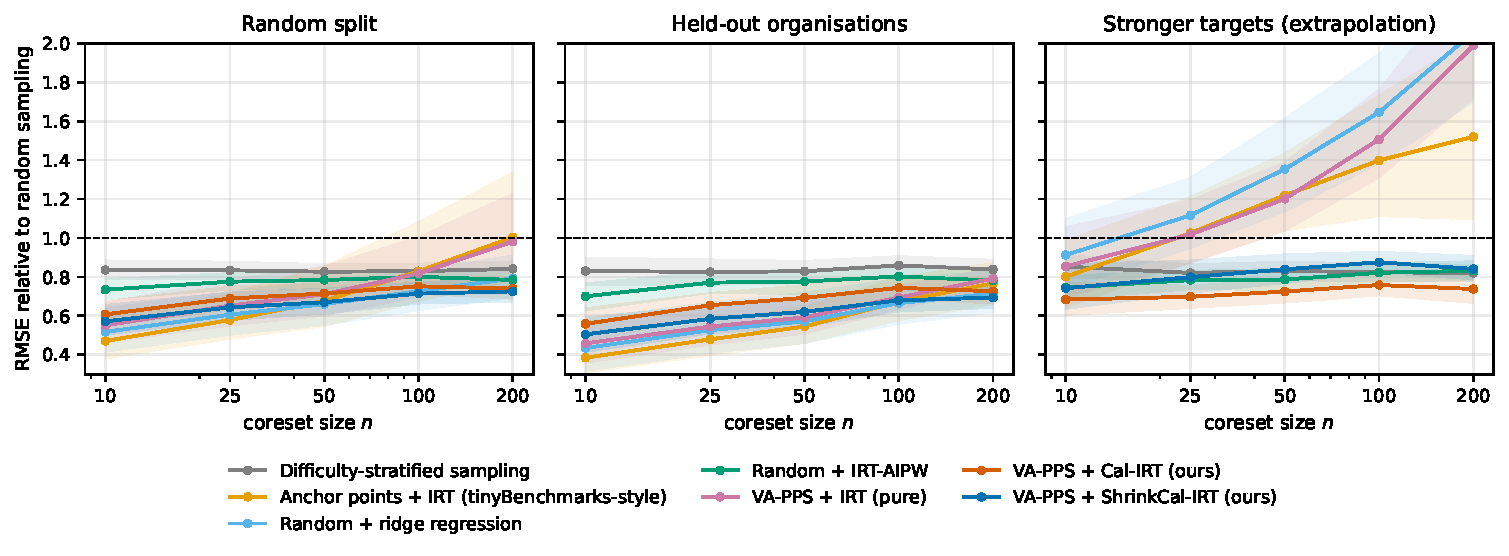
\includegraphics[width=\linewidth]{figs/curves.pdf}
\caption{Relative RMSE vs.\ random sampling as a function of coreset size, per split type (shaded: 95\% CI). The vertical axis is clipped at 2.0; pure-prediction methods continue upwards in the right panel.}
\label{fig:curves}
\end{figure}

\paragraph{Residual correction or recalibration restores robustness.}
Model-assisted (AIPW) estimators remain design-unbiased under any shift: IRT-AIPW with uniform sampling has 0.78 (0.73--0.84) at $n=25$ and 0.82 (0.77--0.87) at $n=100$ under extrapolation and beats random sampling on all 13 benchmarks at both budgets. Cal-IRT with VA-PPS improves on this: 0.70 (0.64--0.76) and 0.76 (0.70--0.82), 13/13 wins, and is better than IRT-AIPW in paired comparisons by 11\% and 8\% (ratio 0.89 and 0.92 with intervals excluding 1; Appendix Table~\ref{tab:pairs}). Under interpolation, Cal-IRT keeps most of the gain (0.69 and 0.75 for random splits), but remains behind the best uncorrected predictors at small $n$ (paired ratio vs.\ ridge 1.14 at $n=25$, CI 1.00--1.34). Its bias under extrapolation is $-0.5$ points versus $-5.2$ for the uncalibrated IRT with the same design (Table~\ref{tab:bias}). ShrinkCal-IRT trades in the other direction: it recovers most of the interpolation advantage (0.64/0.71 for random splits, within the intervals of ridge) and costs 15\% relative to Cal-IRT under extrapolation (0.80/0.88, still better than random sampling on 13/13). No method dominates: the choice between Cal-IRT and ShrinkCal-IRT is a choice about how much extrapolation to expect.

\begin{table}[t]
\caption{Signed error and its share in the MSE at $n=100$: average over benchmarks of the mean signed error $\hat a_t-a_t$ over target models (accuracy points) and bias$^2$/MSE pooled over runs. A shared coreset produces some common-mode error even for unbiased methods.}
\label{tab:bias}
\centering\scriptsize\setlength{\tabcolsep}{3pt}
\begin{tabular}{lcccccc}
\toprule
 & \multicolumn{2}{c}{Random split} & \multicolumn{2}{c}{Held-out organisations} & \multicolumn{2}{c}{Stronger targets (extrapolation)} \\
 & mean err (pts) & bias$^2$/MSE & mean err (pts) & bias$^2$/MSE & mean err (pts) & bias$^2$/MSE \\
\midrule
Random sampling & -0.03 & 28\% & -0.08 & 24\% & -0.09 & 42\% \\
Difficulty-stratified sampling & -0.00 & 4\% & +0.05 & 3\% & -0.13 & 18\% \\
Random + linear calibration & +0.02 & 3\% & -0.02 & 3\% & -2.61 & 64\% \\
Random + ridge regression & +0.11 & 4\% & -0.05 & 3\% & -5.66 & 76\% \\
Anchor points (weighted mean) & -0.35 & 25\% & -1.79 & 26\% & -1.64 & 25\% \\
Anchor points + IRT (tinyBenchmarks-style) & +0.38 & 8\% & -0.20 & 5\% & -5.04 & 73\% \\
D-optimal items + IRT (info-based) & +0.65 & 11\% & -0.44 & 11\% & -5.83 & 77\% \\
Random + IRT (pure) & -0.03 & 4\% & -0.17 & 5\% & -5.23 & 75\% \\
Random + IRT-AIPW & -0.01 & 4\% & +0.02 & 2\% & -0.31 & 18\% \\
VA-PPS + IRT-AIPW & +0.03 & 3\% & -0.04 & 2\% & -0.07 & 14\% \\
VA-PPS + IRT (pure) & +0.17 & 6\% & -0.16 & 4\% & -5.15 & 75\% \\
VA-PPS + Cal-IRT (ours) & -0.04 & 3\% & -0.08 & 2\% & -0.48 & 18\% \\
VA-PPS + ShrinkCal-IRT (ours) & -0.02 & 3\% & -0.11 & 3\% & -1.50 & 31\% \\
AUTO (pseudo-shift, minimax) & +0.01 & 4\% & -0.10 & 3\% & -1.32 & 40\% \\
AUTO (pseudo-shift, mean) & -0.05 & 3\% & -0.08 & 3\% & -1.69 & 45\% \\
\bottomrule
\end{tabular}

\end{table}

\paragraph{Designs matter much less than estimators.}
Holding the estimator fixed, difficulty stratification changes RMSE by $\le4\%$ for IRT-based estimators, and VA-PPS adds at most 5--7\% over stratification, significantly so only in some columns (Appendix Table~\ref{tab:design}; e.g.\ Cal-IRT, VA-PPS vs.\ stratified: 0.96 at $n=25$ and 0.95 at $n=100$ with held-out organisations, 0.93 at $n=25$ under extrapolation, but 0.98--0.99 elsewhere with intervals covering 1). The pure Neyman allocation ($\lambda=1$) is a poor design for estimators that use the Horvitz--Thompson weights alone: the weighted mean with VA-PPS $\lambda=1$ is 9--47\% worse than stratified sampling, and VA-PPS $\lambda=1$ with IRT-AIPW is slightly worse than with $\lambda=0.5$ (0.88 vs 0.78 at $n=100$ under extrapolation; Appendix Table~\ref{tab:abl}). Information-based (D-optimal) item selection, which concentrates items in a few directions of latent space, is worse than random or stratified items for the same estimators in our setting. The IRT dimension ($d\in\{2,4,8\}$) matters little for the corrected estimators; larger $d$ is slightly worse under extrapolation.

\paragraph{Pseudo-shift tuning does not buy robustness.}
Tuning the (design, estimator) pair on pseudo-shifts of the source models (AUTO) does reasonably in the interpolation settings (e.g.\ 0.68/0.75 at $n=25/100$ for random splits, minimax) but is 8--11\% worse than fixed Cal-IRT under extrapolation (paired ratio 1.11, CI 1.04--1.18, at $n=25$; 1.08, CI 1.02--1.15, at $n=100$), and 17--31\% of its minimax choices there are uncorrected predictors (pure IRT, plug-in or ridge; Appendix Table~\ref{tab:auto}), which fail on the real shift. Holding out the top quarter of the \emph{sources} produces a milder gap than the real extrapolation, so the inner validation under-estimates the bias. We view this as a caution against validating shift-robustness only by within-source splits.

\paragraph{Shift severity.}
In a smaller additional run (10 seeds, $n\in\{25,100\}$, four designs; Appendix~\ref{app:shift}) we varied which models are targets: the strongest 10\% or 50\% of models, or the weakest 25\%. Uncorrected predictors fail in every direction of extrapolation, and most when the sources are only the weaker half: at $n=100$ pure IRT is 1.16 (1.04--1.36) of random-sampling RMSE for the strongest-10\% targets and 2.07 (1.77--2.49) for strongest-50\%, and for the weakest-25\% targets they over-predict by 8--9 points (relative RMSE 2.1). Cal-IRT is below 1 in all four settings at both budgets, but for the weakest-25\% targets its intervals include 1 (0.90, 0.77--1.06 at $n=25$; 0.92, 0.81--1.05 at $n=100$) and so does IRT-AIPW's, so we cannot claim a gain over random sampling there; difficulty-stratified sampling (0.92 and 0.90) is the only method whose interval stays at or below 1.


\paragraph{Number of source models.}
In a further run on 7 benchmarks (10 seeds, $n\in\{25,100\}$, stratified and VA-PPS designs) we kept only $m\in\{20,50,100\}$ randomly chosen source models (Appendix~\ref{app:src}). With $m=20$, all model-based methods are clearly weaker, and under extrapolation difficulty-stratified sampling (0.79 at $n=25$, 0.83 at $n=100$) is better than all of them (Cal-IRT 0.86 and 0.94, intervals covering 1 at $n=100$); with $m=50$ Cal-IRT is already at 0.76 / 0.85 and with all sources 0.68 / 0.73 under extrapolation. Interpolation gains of uncorrected predictors also need $m\gtrsim50$ (ridge 0.71 / 0.56 / 0.52 at $n=25$ for $m=20/50/100$). The same figures are in a table in the appendix; note that for the HELM benchmarks the number of available source models is below 100, so $m=100$ equals the full source set there.

\section{Discussion and limitations}
\label{sec:discussion}
\paragraph{What the evidence supports.}
On these 13 binary benchmarks, (i) a model-free change of design (difficulty stratification using source records) gives a consistent $\sim$17\% RMSE reduction; (ii) learned predictors give large further gains when the target is an interpolation of the source population, and become worse than random sampling---through a systematic downward bias---when the targets are stronger than every source model; (iii) per-target recalibration of an IRT predictor (Cal-IRT) or its pretest-shrunk version (ShrinkCal-IRT) retains much of the interpolation gain while staying better than random sampling in all our extrapolation settings, and Cal-IRT beats the AIPW estimator by 6--15\% in paired comparisons; (iv) the contribution of the variance-aware design is small ($\le$5--7\%, not always distinguishable from zero), and the uniform floor ($\lambda<1$) is safer; (v) selecting among methods by pseudo-shift validation inside the source set was not effective. In sample-size terms, and assuming the error of random sampling scales as $n^{-1/2}$, a relative RMSE of 0.70--0.76 corresponds to the accuracy of $\approx$1.7--2$\times$ as many random items. Practical reading: if one cannot rule out that a new model lies outside the span of the source models---the usual case for a new, stronger model---an uncorrected predictor can be worse than simply running random items, and a corrected or recalibrated estimator on a difficulty-stratified or VA-PPS coreset is the safer default; if the target is a sibling of known models, uncorrected predictors (or ShrinkCal-IRT) are better.

\paragraph{Limitations.}
\emph{Scope.} Only binary correctness on 13 benchmark matrices from two sources was studied; continuous or open-ended scores, chat/judge benchmarks and benchmarks with very few source models are not covered. The HELM benchmarks have only 79--83 models (about 20 targets per split), so their results are noisier. \emph{Shift is operationalised, not measured.} ``Stronger targets'' (top 25\% by accuracy) is one particular, fairly severe extrapolation; the ordering of methods under milder or different shifts (other capability profiles, different eras of models, new architectures) may differ, and the split is deterministic, so the intervals do not account for which models are strongest. Leaderboard models include many fine-tunes and merges of a few base models, which flatters interpolation (organisation hold-out only partly addresses this). \emph{Target accuracy is on the benchmark itself.} All targets are scored on the same finite item set; we say nothing about generalisation to unseen items, nor about evaluation noise in the underlying leaderboards (e.g.\ sampling temperature, prompt format). \emph{Baselines are re-implementations.} Anchor Points, tinyBenchmarks-style, D-optimal/metabench-style and AIPW baselines are our own simplified versions on binary data (e.g.\ $k$-means on binary vectors instead of confidence-based clustering, a fixed IRT dimension, no cross-validated mixing weights); they are not the original authors' code, and stronger tuned versions may close some gaps. \emph{Tuning.} IRT regularisation, the ability prior, the Platt penalty and $c_0$ were set on a separate development run using 9--11 of the benchmarks and fixed values; $c_0=0.5$ was not varied in the main run, and the VA-PPS $\lambda$ was fixed to the value that looked best for Cal-IRT in development, which turned out to be a worse choice than $\lambda=0.5$ for AIPW-type estimators. \emph{No guarantees.} Cal-IRT and ShrinkCal-IRT are heuristics: they are not unbiased (Cal-IRT has a small negative bias under extrapolation, $-0.5$ points), the shrinkage is a pretest rule without formal risk guarantees, and Proposition~\ref{prop:neyman} concerns Poisson sampling and a fixed predictor while we use systematic sampling with a proxy variance. \emph{Metric.} Relative RMSE averages errors over target models sharing a single coreset; ranking metrics are computed within a split and are not comparable across split types. \emph{Cost.} IRT fitting on the largest benchmark takes on the order of 10--30\,s per source set on one CPU core; per-target inference is negligible.

\paragraph{Broader impact.} Cheaper evaluation lowers costs, but over-trusting a predicted score (particularly for new, stronger models) can mislead model comparison; we recommend reporting the coreset size and an uncertainty interval, and not using predicted scores for decisions near ties.


\bibliographystyle{plainnat}
\bibliography{refs}

\appendix
\section{Data}
\begin{table}[h]
\caption{Item-level matrices used (OLL: Open LLM Leaderboard v2; HELM). ``const.\ items'': items answered identically by all models. Accuracy statistics are over models.}
\label{tab:data}
\centering\scriptsize\begin{tabular}{llrrrrrr}
\toprule
benchmark & source & models & items & mean acc. & sd acc. & range & const.\ items \\
\midrule
arc challenge & OLL & 218 & 1172 & 52.2 & 12.9 & 20.5--75.1 & 32 \\
bbh & OLL & 446 & 5761 & 44.7 & 11.6 & 24.1--74.7 & 0 \\
gpqa & OLL & 447 & 1192 & 28.9 & 3.8 & 22.5--43.7 & 0 \\
ifeval & OLL & 448 & 541 & 33.3 & 20.4 & 3.7--88.0 & 7 \\
mmlu pro & OLL & 448 & 12032 & 28.1 & 12.9 & 10.3--59.7 & 1 \\
musr & OLL & 448 & 756 & 39.9 & 4.1 & 32.3--53.6 & 10 \\
openllm math & OLL & 447 & 894 & 5.1 & 6.8 & 0.0--35.6 & 119 \\
commonsense & HELM & 83 & 500 & 82.3 & 17.3 & 22.2--97.2 & 0 \\
gsm & HELM & 83 & 1000 & 65.7 & 24.9 & 2.8--95.6 & 3 \\
legalbench & HELM & 79 & 2047 & 53.3 & 10.6 & 22.8--70.2 & 53 \\
math & HELM & 83 & 437 & 56.8 & 27.4 & 2.5--93.4 & 1 \\
med qa & HELM & 83 & 1000 & 59.4 & 16.4 & 21.5--86.9 & 2 \\
mmlu & HELM & 83 & 567 & 61.3 & 12.4 & 22.9--81.1 & 1 \\
\bottomrule
\end{tabular}

\end{table}
\begin{table}[h]
\caption{Absolute RMSE (accuracy points; $\sqrt{\text{seed-averaged MSE}}$) at $n=100$ for random splits and stronger targets.}
\label{tab:abs}
\centering\tiny\setlength{\tabcolsep}{2pt}\begin{tabular}{llrrrrrrrrrrrrr}
\toprule
split & method & arc challenge & bbh & commonsense & gpqa & gsm & ifeval & legalbench & math & med qa & mmlu & mmlu pro & musr & openllm math \\
\midrule
random & Random sampling & 4.4 & 4.6 & 3.1 & 4.2 & 3.9 & 3.8 & 4.8 & 3.5 & 4.7 & 4.0 & 4.1 & 4.1 & 1.9 \\
random & Difficulty-stratified sampling & 3.3 & 4.1 & 2.4 & 4.1 & 3.3 & 3.2 & 3.5 & 3.0 & 3.7 & 3.0 & 3.5 & 3.6 & 1.7 \\
random & Random + IRT-AIPW & 3.1 & 3.7 & 2.7 & 3.7 & 3.2 & 3.0 & 3.4 & 3.0 & 3.5 & 3.1 & 3.3 & 3.2 & 1.7 \\
random & VA-PPS + Cal-IRT (ours) & 2.8 & 3.5 & 2.5 & 3.5 & 3.1 & 2.9 & 3.3 & 3.2 & 3.5 & 2.9 & 3.1 & 2.8 & 1.3 \\
random & VA-PPS + ShrinkCal-IRT (ours) & 2.5 & 3.0 & 2.6 & 3.0 & 3.3 & 2.8 & 3.3 & 3.3 & 3.5 & 2.9 & 2.8 & 2.4 & 1.3 \\
top & Random sampling & 4.4 & 4.6 & 1.9 & 4.5 & 2.7 & 4.0 & 5.0 & 3.0 & 4.3 & 3.9 & 4.5 & 4.1 & 3.3 \\
top & Difficulty-stratified sampling & 3.2 & 4.0 & 1.6 & 3.9 & 2.4 & 3.7 & 3.4 & 2.4 & 3.0 & 2.9 & 4.0 & 3.8 & 3.0 \\
top & Random + IRT-AIPW & 2.9 & 4.0 & 1.8 & 4.1 & 2.3 & 3.5 & 3.3 & 2.7 & 3.2 & 2.8 & 4.1 & 3.2 & 3.0 \\
top & VA-PPS + Cal-IRT (ours) & 2.8 & 3.6 & 1.3 & 3.8 & 2.3 & 3.5 & 2.9 & 2.3 & 3.4 & 2.5 & 4.1 & 3.0 & 2.8 \\
top & VA-PPS + ShrinkCal-IRT (ours) & 3.2 & 4.0 & 1.8 & 4.1 & 2.7 & 3.8 & 3.4 & 2.8 & 3.9 & 3.1 & 4.4 & 3.3 & 3.2 \\
\bottomrule
\end{tabular}

\end{table}

\section{Implementation details}\label{app:impl}
\textbf{IRT.} $P(y_{ji}=1)=\sigma(\theta_j^\top\alpha_i+\beta_i)$, minimised over $(\theta,\alpha,\beta)$ with scipy L-BFGS-B (max.\ 150 iterations, 20 correction pairs, float32 matrix products) on the sum of binary cross-entropies plus $\frac12\|\theta\|^2+\frac12\|\alpha\|^2+0.05\|\beta-\beta^{0}\|^2$, where $\beta^{0}_i=\mathrm{logit}(\mathrm{clip}(\bar p_i,0.02,0.98))$ and initial $\theta,\alpha\sim 0.1\,\mathcal N(0,I)$. Target ability: MAP with prior $\mathcal N(0,4I)$ by batched damped Newton iterations (step clipped to $\pm2$, at most 25 iterations). Platt recalibration: two-parameter Newton (at most 20 iterations, steps clipped to $\pm1$) on the coreset, ridge penalty 1 towards $(s,c)=(1,0)$. ShrinkCal: $\hat v_t=\mathrm{Var}_C(y-\hat p)/n\cdot(1-n/N)$ (unbiased sample variance), $c_0=0.5$.\\
\textbf{VA-PPS.} $v_i$ is the mean squared residual of the $d=4$ IRT fit on the source models; $s_i=\sqrt{\max(v_i,10^{-4})}$; inclusion probabilities by water-filling to $\sum\pi_i=n$; systematic sampling over difficulty-sorted items (ties broken at random) with a uniformly random start.\\
\textbf{Anchor points.} scikit-learn \texttt{KMeans} with $k=n$, \texttt{n\_init}=1, \texttt{max\_iter}=30 on the source item vectors; the item closest to each centroid is the anchor, weight = cluster size$/N$.\\
\textbf{D-optimal.} Greedy $\log\det$ maximisation of $I+\sum_i \bar w_i\alpha_i\alpha_i^\top$ with $\bar w_i=\overline{p(1-p)}$ over source models, via Sherman--Morrison updates.\\
\textbf{Ridge.} \texttt{RidgeCV}, $\alpha\in\{10^{-2},\dots,10^{3}\}$ (12 values), source coreset responses $\to$ source full accuracy.\\
\textbf{Cross-fitting.} 5 folds over coreset items.\\
\textbf{AUTO.} Inner splits use seed-dependent random permutations; 2 repetitions of coreset draws per inner split; inner IRT fits are refitted on the inner source subset.

\section{Additional results}
\begin{table}[h]
\caption{Relative RMSE at all five budgets (same format as Table~\ref{tab:main}); columns are protocol$\times n$ in the order $n=10,25,50,100,200$.}\label{tab:full}
\centering\tiny\setlength{\tabcolsep}{1.5pt}\resizebox{\linewidth}{!}{\begin{tabular}{lccccccccccccccc}
\toprule
 & \multicolumn{5}{c}{Random split} & \multicolumn{5}{c}{Held-out organisations} & \multicolumn{5}{c}{Stronger targets (extrapolation)} \\
 & $n$=10 & $n$=25 & $n$=50 & $n$=100 & $n$=200 & $n$=10 & $n$=25 & $n$=50 & $n$=100 & $n$=200 & $n$=10 & $n$=25 & $n$=50 & $n$=100 & $n$=200 \\
\midrule
Random sampling & 1.00\,\scriptsize(1.00--1.00) & 1.00\,\scriptsize(1.00--1.00) & 1.00\,\scriptsize(1.00--1.00) & 1.00\,\scriptsize(1.00--1.00) & 1.00\,\scriptsize(1.00--1.00) & 1.00\,\scriptsize(1.00--1.00) & 1.00\,\scriptsize(1.00--1.00) & 1.00\,\scriptsize(1.00--1.00) & 1.00\,\scriptsize(1.00--1.00) & 1.00\,\scriptsize(1.00--1.00) & 1.00\,\scriptsize(1.00--1.00) & 1.00\,\scriptsize(1.00--1.00) & 1.00\,\scriptsize(1.00--1.00) & 1.00\,\scriptsize(1.00--1.00) & 1.00\,\scriptsize(1.00--1.00) \\
Difficulty-stratified sampling & 0.84\,\scriptsize(0.79--0.88) & 0.83\,\scriptsize(0.79--0.88) & 0.83\,\scriptsize(0.79--0.87) & 0.83\,\scriptsize(0.79--0.87) & 0.84\,\scriptsize(0.80--0.88) & 0.83\,\scriptsize(0.76--0.91) & 0.83\,\scriptsize(0.76--0.89) & 0.83\,\scriptsize(0.77--0.89) & 0.86\,\scriptsize(0.80--0.91) & 0.84\,\scriptsize(0.79--0.89) & 0.85\,\scriptsize(0.80--0.92) & 0.82\,\scriptsize(0.78--0.87) & 0.83\,\scriptsize(0.78--0.88) & 0.82\,\scriptsize(0.78--0.87) & 0.82\,\scriptsize(0.78--0.86) \\
Random + linear calibration & 0.56\,\scriptsize(0.45--0.68) & 0.67\,\scriptsize(0.57--0.76) & 0.73\,\scriptsize(0.65--0.80) & 0.79\,\scriptsize(0.74--0.83) & 0.81\,\scriptsize(0.76--0.85) & 0.48\,\scriptsize(0.35--0.65) & 0.61\,\scriptsize(0.49--0.75) & 0.68\,\scriptsize(0.58--0.81) & 0.77\,\scriptsize(0.69--0.85) & 0.79\,\scriptsize(0.73--0.84) & 0.85\,\scriptsize(0.72--1.00) & 0.95\,\scriptsize(0.85--1.07) & 1.01\,\scriptsize(0.90--1.15) & 1.07\,\scriptsize(0.95--1.19) & 1.06\,\scriptsize(0.97--1.18) \\
Random + ridge regression & 0.52\,\scriptsize(0.41--0.64) & 0.61\,\scriptsize(0.50--0.72) & 0.66\,\scriptsize(0.55--0.78) & 0.73\,\scriptsize(0.63--0.83) & 0.79\,\scriptsize(0.68--0.91) & 0.43\,\scriptsize(0.32--0.60) & 0.53\,\scriptsize(0.41--0.67) & 0.57\,\scriptsize(0.46--0.73) & 0.67\,\scriptsize(0.56--0.81) & 0.71\,\scriptsize(0.62--0.85) & 0.91\,\scriptsize(0.73--1.11) & 1.12\,\scriptsize(0.94--1.32) & 1.35\,\scriptsize(1.13--1.61) & 1.65\,\scriptsize(1.37--1.96) & 2.06\,\scriptsize(1.68--2.52) \\
Anchor points (weighted mean) & 0.68\,\scriptsize(0.60--0.76) & 0.78\,\scriptsize(0.68--0.89) & 0.91\,\scriptsize(0.79--1.06) & 1.08\,\scriptsize(0.91--1.28) & 1.28\,\scriptsize(1.09--1.53) & 0.67\,\scriptsize(0.55--0.81) & 0.82\,\scriptsize(0.67--1.03) & 0.94\,\scriptsize(0.76--1.23) & 1.21\,\scriptsize(0.95--1.63) & 1.41\,\scriptsize(1.09--1.87) & 0.72\,\scriptsize(0.56--1.00) & 0.90\,\scriptsize(0.65--1.30) & 1.08\,\scriptsize(0.76--1.62) & 1.34\,\scriptsize(0.90--2.07) & 1.67\,\scriptsize(1.06--2.62) \\
Anchor points + IRT (tinyBenchmarks-style) & 0.47\,\scriptsize(0.37--0.59) & 0.58\,\scriptsize(0.47--0.71) & 0.68\,\scriptsize(0.54--0.85) & 0.83\,\scriptsize(0.66--1.07) & 1.00\,\scriptsize(0.78--1.33) & 0.38\,\scriptsize(0.31--0.48) & 0.48\,\scriptsize(0.40--0.58) & 0.54\,\scriptsize(0.46--0.65) & 0.67\,\scriptsize(0.58--0.81) & 0.77\,\scriptsize(0.66--0.88) & 0.80\,\scriptsize(0.63--0.99) & 1.02\,\scriptsize(0.85--1.22) & 1.22\,\scriptsize(1.03--1.43) & 1.40\,\scriptsize(1.11--1.73) & 1.52\,\scriptsize(1.08--2.05) \\
D-optimal items + IRT (info-based) & 0.56\,\scriptsize(0.43--0.73) & 0.70\,\scriptsize(0.55--0.92) & 0.83\,\scriptsize(0.64--1.10) & 1.01\,\scriptsize(0.79--1.33) & 1.19\,\scriptsize(0.92--1.59) & 0.43\,\scriptsize(0.32--0.55) & 0.53\,\scriptsize(0.41--0.67) & 0.61\,\scriptsize(0.48--0.76) & 0.77\,\scriptsize(0.63--0.96) & 0.89\,\scriptsize(0.73--1.09) & 0.77\,\scriptsize(0.62--0.96) & 1.01\,\scriptsize(0.85--1.20) & 1.28\,\scriptsize(1.07--1.53) & 1.62\,\scriptsize(1.33--1.98) & 2.00\,\scriptsize(1.58--2.55) \\
Random + IRT (pure) & 0.56\,\scriptsize(0.46--0.67) & 0.65\,\scriptsize(0.55--0.75) & 0.69\,\scriptsize(0.60--0.80) & 0.78\,\scriptsize(0.70--0.86) & 0.91\,\scriptsize(0.81--1.02) & 0.48\,\scriptsize(0.37--0.61) & 0.57\,\scriptsize(0.46--0.69) & 0.61\,\scriptsize(0.52--0.73) & 0.71\,\scriptsize(0.64--0.80) & 0.81\,\scriptsize(0.76--0.87) & 0.92\,\scriptsize(0.72--1.14) & 1.08\,\scriptsize(0.90--1.29) & 1.25\,\scriptsize(1.08--1.46) & 1.54\,\scriptsize(1.35--1.79) & 2.05\,\scriptsize(1.76--2.42) \\
Random + IRT-AIPW & 0.73\,\scriptsize(0.68--0.79) & 0.78\,\scriptsize(0.73--0.82) & 0.78\,\scriptsize(0.74--0.83) & 0.80\,\scriptsize(0.77--0.83) & 0.78\,\scriptsize(0.74--0.82) & 0.70\,\scriptsize(0.63--0.77) & 0.77\,\scriptsize(0.71--0.83) & 0.78\,\scriptsize(0.71--0.84) & 0.80\,\scriptsize(0.74--0.86) & 0.78\,\scriptsize(0.73--0.83) & 0.74\,\scriptsize(0.68--0.81) & 0.78\,\scriptsize(0.73--0.84) & 0.79\,\scriptsize(0.73--0.84) & 0.82\,\scriptsize(0.77--0.87) & 0.83\,\scriptsize(0.78--0.88) \\
VA-PPS + IRT-AIPW & 0.74\,\scriptsize(0.68--0.81) & 0.78\,\scriptsize(0.72--0.87) & 0.80\,\scriptsize(0.74--0.87) & 0.82\,\scriptsize(0.77--0.89) & 0.80\,\scriptsize(0.74--0.89) & 0.71\,\scriptsize(0.63--0.81) & 0.75\,\scriptsize(0.68--0.83) & 0.74\,\scriptsize(0.68--0.80) & 0.77\,\scriptsize(0.71--0.82) & 0.76\,\scriptsize(0.71--0.82) & 0.72\,\scriptsize(0.65--0.80) & 0.76\,\scriptsize(0.69--0.84) & 0.80\,\scriptsize(0.72--0.89) & 0.88\,\scriptsize(0.78--0.98) & 0.84\,\scriptsize(0.73--0.96) \\
VA-PPS + IRT (pure) & 0.55\,\scriptsize(0.45--0.67) & 0.65\,\scriptsize(0.54--0.79) & 0.71\,\scriptsize(0.60--0.85) & 0.82\,\scriptsize(0.69--1.00) & 0.98\,\scriptsize(0.81--1.23) & 0.46\,\scriptsize(0.36--0.58) & 0.54\,\scriptsize(0.45--0.64) & 0.59\,\scriptsize(0.51--0.68) & 0.69\,\scriptsize(0.64--0.76) & 0.79\,\scriptsize(0.74--0.85) & 0.85\,\scriptsize(0.68--1.07) & 1.02\,\scriptsize(0.86--1.20) & 1.20\,\scriptsize(1.04--1.40) & 1.51\,\scriptsize(1.30--1.76) & 1.99\,\scriptsize(1.71--2.35) \\
VA-PPS + Cal-IRT (ours) & 0.61\,\scriptsize(0.54--0.68) & 0.69\,\scriptsize(0.63--0.75) & 0.71\,\scriptsize(0.67--0.77) & 0.75\,\scriptsize(0.71--0.80) & 0.74\,\scriptsize(0.68--0.80) & 0.56\,\scriptsize(0.47--0.64) & 0.65\,\scriptsize(0.59--0.72) & 0.69\,\scriptsize(0.62--0.76) & 0.74\,\scriptsize(0.69--0.80) & 0.73\,\scriptsize(0.66--0.79) & 0.68\,\scriptsize(0.60--0.77) & 0.70\,\scriptsize(0.64--0.76) & 0.72\,\scriptsize(0.67--0.79) & 0.76\,\scriptsize(0.70--0.82) & 0.74\,\scriptsize(0.66--0.82) \\
VA-PPS + ShrinkCal-IRT (ours) & 0.57\,\scriptsize(0.50--0.66) & 0.64\,\scriptsize(0.58--0.72) & 0.67\,\scriptsize(0.61--0.74) & 0.71\,\scriptsize(0.66--0.77) & 0.73\,\scriptsize(0.67--0.80) & 0.50\,\scriptsize(0.41--0.59) & 0.58\,\scriptsize(0.51--0.65) & 0.62\,\scriptsize(0.54--0.69) & 0.68\,\scriptsize(0.62--0.74) & 0.69\,\scriptsize(0.64--0.75) & 0.74\,\scriptsize(0.62--0.87) & 0.80\,\scriptsize(0.71--0.90) & 0.84\,\scriptsize(0.76--0.92) & 0.88\,\scriptsize(0.82--0.93) & 0.84\,\scriptsize(0.78--0.91) \\
AUTO (pseudo-shift, minimax) & 0.58\,\scriptsize(0.48--0.69) & 0.68\,\scriptsize(0.59--0.76) & 0.71\,\scriptsize(0.64--0.79) & 0.75\,\scriptsize(0.71--0.80) & 0.79\,\scriptsize(0.71--0.90) & 0.51\,\scriptsize(0.38--0.66) & 0.62\,\scriptsize(0.51--0.73) & 0.67\,\scriptsize(0.58--0.75) & 0.73\,\scriptsize(0.67--0.78) & 0.72\,\scriptsize(0.66--0.79) & 0.72\,\scriptsize(0.61--0.84) & 0.77\,\scriptsize(0.68--0.87) & 0.83\,\scriptsize(0.74--0.91) & 0.82\,\scriptsize(0.74--0.91) & 0.83\,\scriptsize(0.74--0.95) \\
AUTO (pseudo-shift, mean) & 0.55\,\scriptsize(0.44--0.68) & 0.66\,\scriptsize(0.55--0.76) & 0.70\,\scriptsize(0.61--0.78) & 0.72\,\scriptsize(0.67--0.77) & 0.78\,\scriptsize(0.70--0.89) & 0.47\,\scriptsize(0.35--0.62) & 0.58\,\scriptsize(0.45--0.72) & 0.62\,\scriptsize(0.52--0.72) & 0.70\,\scriptsize(0.63--0.77) & 0.71\,\scriptsize(0.65--0.77) & 0.75\,\scriptsize(0.63--0.87) & 0.81\,\scriptsize(0.71--0.95) & 0.85\,\scriptsize(0.76--0.97) & 0.87\,\scriptsize(0.76--0.99) & 0.83\,\scriptsize(0.73--0.96) \\
\bottomrule
\end{tabular}
}
\end{table}
\begin{table}[h]
\caption{Spearman correlation between predicted and true accuracy of the target models in a split (mean over benchmarks and seeds; in parentheses the difference to random sampling with its 95\% hierarchical-bootstrap interval).}\label{tab:spearman}
\centering\tiny\setlength{\tabcolsep}{1.5pt}\resizebox{\linewidth}{!}{\begin{tabular}{lcccccc}
\toprule
 & \multicolumn{2}{c}{Random split} & \multicolumn{2}{c}{Held-out organisations} & \multicolumn{2}{c}{Stronger targets (extrapolation)} \\
 & $n$=25 & $n$=100 & $n$=25 & $n$=100 & $n$=25 & $n$=100 \\
\midrule
Random sampling & 0.795 & 0.910 & 0.726 & 0.871 & 0.532 & 0.759 \\
Difficulty-stratified sampling & 0.784\,\scriptsize(-0.011; -0.036..+0.006) & 0.913\,\scriptsize(+0.003; -0.008..+0.015) & 0.737\,\scriptsize(+0.011; -0.010..+0.032) & 0.873\,\scriptsize(+0.002; -0.010..+0.016) & 0.536\,\scriptsize(+0.004; -0.030..+0.038) & 0.774\,\scriptsize(+0.015; -0.007..+0.039) \\
Random + linear calibration & 0.795\,\scriptsize(+0.000; +0.000..+0.000) & 0.910\,\scriptsize(+0.000; +0.000..+0.000) & 0.726\,\scriptsize(+0.000; +0.000..+0.000) & 0.871\,\scriptsize(+0.000; +0.000..+0.000) & 0.529\,\scriptsize(-0.003; -0.008..+0.000) & 0.759\,\scriptsize(+0.000; +0.000..+0.000) \\
Random + ridge regression & 0.854\,\scriptsize(+0.059; +0.019..+0.108) & 0.941\,\scriptsize(+0.031; +0.001..+0.073) & 0.817\,\scriptsize(+0.091; +0.022..+0.173) & 0.922\,\scriptsize(+0.051; +0.004..+0.113) & 0.404\,\scriptsize(-0.128; -0.202..-0.064) & 0.624\,\scriptsize(-0.135; -0.200..-0.064) \\
Anchor points (weighted mean) & 0.844\,\scriptsize(+0.048; +0.004..+0.078) & 0.899\,\scriptsize(-0.011; -0.054..+0.017) & 0.776\,\scriptsize(+0.049; -0.011..+0.090) & 0.835\,\scriptsize(-0.036; -0.118..+0.020) & 0.481\,\scriptsize(-0.050; -0.098..-0.002) & 0.701\,\scriptsize(-0.058; -0.120..+0.007) \\
Anchor points + IRT (tinyBenchmarks-style) & 0.892\,\scriptsize(+0.097; +0.056..+0.143) & 0.947\,\scriptsize(+0.037; +0.014..+0.069) & 0.854\,\scriptsize(+0.128; +0.075..+0.189) & 0.921\,\scriptsize(+0.051; +0.019..+0.091) & 0.403\,\scriptsize(-0.128; -0.216..-0.049) & 0.680\,\scriptsize(-0.079; -0.219..+0.055) \\
D-optimal items + IRT (info-based) & 0.879\,\scriptsize(+0.084; +0.040..+0.132) & 0.938\,\scriptsize(+0.029; +0.000..+0.067) & 0.856\,\scriptsize(+0.130; +0.063..+0.201) & 0.918\,\scriptsize(+0.047; +0.005..+0.099) & 0.415\,\scriptsize(-0.117; -0.262..+0.009) & 0.603\,\scriptsize(-0.156; -0.334..-0.012) \\
Random + IRT (pure) & 0.841\,\scriptsize(+0.046; +0.020..+0.077) & 0.930\,\scriptsize(+0.020; +0.004..+0.042) & 0.788\,\scriptsize(+0.062; +0.021..+0.107) & 0.898\,\scriptsize(+0.027; +0.005..+0.055) & 0.407\,\scriptsize(-0.125; -0.191..-0.059) & 0.614\,\scriptsize(-0.146; -0.248..-0.051) \\
Random + IRT-AIPW & 0.803\,\scriptsize(+0.007; +0.000..+0.015) & 0.917\,\scriptsize(+0.008; +0.001..+0.018) & 0.733\,\scriptsize(+0.007; -0.001..+0.018) & 0.882\,\scriptsize(+0.011; +0.001..+0.026) & 0.515\,\scriptsize(-0.017; -0.027..-0.005) & 0.760\,\scriptsize(+0.000; -0.009..+0.013) \\
VA-PPS + IRT-AIPW & 0.820\,\scriptsize(+0.024; +0.009..+0.039) & 0.925\,\scriptsize(+0.016; +0.004..+0.032) & 0.760\,\scriptsize(+0.034; +0.019..+0.051) & 0.896\,\scriptsize(+0.025; +0.008..+0.047) & 0.551\,\scriptsize(+0.020; -0.009..+0.054) & 0.777\,\scriptsize(+0.017; -0.007..+0.048) \\
VA-PPS + IRT (pure) & 0.854\,\scriptsize(+0.059; +0.031..+0.090) & 0.934\,\scriptsize(+0.024; +0.006..+0.050) & 0.808\,\scriptsize(+0.082; +0.044..+0.124) & 0.903\,\scriptsize(+0.032; +0.011..+0.062) & 0.436\,\scriptsize(-0.096; -0.169..-0.031) & 0.642\,\scriptsize(-0.117; -0.214..-0.023) \\
VA-PPS + Cal-IRT (ours) & 0.832\,\scriptsize(+0.036; +0.020..+0.054) & 0.930\,\scriptsize(+0.020; +0.007..+0.039) & 0.776\,\scriptsize(+0.050; +0.029..+0.074) & 0.899\,\scriptsize(+0.029; +0.009..+0.054) & 0.555\,\scriptsize(+0.024; -0.004..+0.058) & 0.787\,\scriptsize(+0.028; +0.004..+0.059) \\
VA-PPS + ShrinkCal-IRT (ours) & 0.848\,\scriptsize(+0.052; +0.030..+0.075) & 0.937\,\scriptsize(+0.027; +0.009..+0.052) & 0.800\,\scriptsize(+0.074; +0.042..+0.113) & 0.911\,\scriptsize(+0.040; +0.013..+0.073) & 0.546\,\scriptsize(+0.014; -0.015..+0.052) & 0.784\,\scriptsize(+0.024; +0.001..+0.056) \\
AUTO (pseudo-shift, minimax) & 0.831\,\scriptsize(+0.036; +0.016..+0.058) & 0.929\,\scriptsize(+0.019; +0.004..+0.040) & 0.787\,\scriptsize(+0.060; +0.028..+0.101) & 0.903\,\scriptsize(+0.032; +0.007..+0.063) & 0.528\,\scriptsize(-0.004; -0.037..+0.034) & 0.774\,\scriptsize(+0.015; -0.023..+0.053) \\
\bottomrule
\end{tabular}
}
\end{table}
\begin{table}[h]
\caption{Kendall $\tau$, same format as Table~\ref{tab:spearman}.}\label{tab:kendall}
\centering\tiny\setlength{\tabcolsep}{1.5pt}\resizebox{\linewidth}{!}{\begin{tabular}{lcccccc}
\toprule
 & \multicolumn{2}{c}{Random split} & \multicolumn{2}{c}{Held-out organisations} & \multicolumn{2}{c}{Stronger targets (extrapolation)} \\
 & $n$=25 & $n$=100 & $n$=25 & $n$=100 & $n$=25 & $n$=100 \\
\midrule
Random sampling & 0.660 & 0.798 & 0.588 & 0.742 & 0.413 & 0.612 \\
Difficulty-stratified sampling & 0.653\,\scriptsize(-0.007; -0.027..+0.008) & 0.801\,\scriptsize(+0.004; -0.007..+0.015) & 0.600\,\scriptsize(+0.012; -0.006..+0.031) & 0.744\,\scriptsize(+0.002; -0.010..+0.015) & 0.416\,\scriptsize(+0.003; -0.026..+0.032) & 0.625\,\scriptsize(+0.013; -0.004..+0.035) \\
Random + linear calibration & 0.660\,\scriptsize(+0.000; +0.000..+0.000) & 0.798\,\scriptsize(+0.000; +0.000..+0.000) & 0.588\,\scriptsize(+0.000; +0.000..+0.000) & 0.742\,\scriptsize(+0.000; +0.000..+0.000) & 0.411\,\scriptsize(-0.002; -0.006..+0.000) & 0.612\,\scriptsize(+0.000; +0.000..+0.000) \\
Random + ridge regression & 0.696\,\scriptsize(+0.035; +0.004..+0.075) & 0.822\,\scriptsize(+0.024; -0.006..+0.064) & 0.649\,\scriptsize(+0.061; +0.008..+0.124) & 0.786\,\scriptsize(+0.045; -0.001..+0.099) & 0.293\,\scriptsize(-0.120; -0.180..-0.070) & 0.471\,\scriptsize(-0.141; -0.198..-0.081) \\
Anchor points (weighted mean) & 0.707\,\scriptsize(+0.047; +0.006..+0.075) & 0.794\,\scriptsize(-0.004; -0.045..+0.027) & 0.633\,\scriptsize(+0.045; -0.007..+0.083) & 0.716\,\scriptsize(-0.026; -0.100..+0.028) & 0.351\,\scriptsize(-0.063; -0.103..-0.024) & 0.542\,\scriptsize(-0.069; -0.127..-0.008) \\
Anchor points + IRT (tinyBenchmarks-style) & 0.747\,\scriptsize(+0.087; +0.054..+0.120) & 0.840\,\scriptsize(+0.042; +0.020..+0.069) & 0.698\,\scriptsize(+0.111; +0.075..+0.148) & 0.797\,\scriptsize(+0.056; +0.030..+0.083) & 0.290\,\scriptsize(-0.123; -0.188..-0.063) & 0.527\,\scriptsize(-0.084; -0.189..+0.027) \\
D-optimal items + IRT (info-based) & 0.725\,\scriptsize(+0.065; +0.030..+0.103) & 0.823\,\scriptsize(+0.025; -0.003..+0.058) & 0.694\,\scriptsize(+0.106; +0.055..+0.155) & 0.784\,\scriptsize(+0.043; +0.004..+0.085) & 0.310\,\scriptsize(-0.103; -0.205..-0.006) & 0.473\,\scriptsize(-0.139; -0.270..-0.025) \\
Random + IRT (pure) & 0.685\,\scriptsize(+0.025; +0.004..+0.049) & 0.812\,\scriptsize(+0.015; -0.000..+0.033) & 0.624\,\scriptsize(+0.037; +0.005..+0.067) & 0.762\,\scriptsize(+0.020; +0.000..+0.043) & 0.296\,\scriptsize(-0.117; -0.170..-0.064) & 0.468\,\scriptsize(-0.144; -0.218..-0.068) \\
Random + IRT-AIPW & 0.647\,\scriptsize(-0.013; -0.019..-0.005) & 0.797\,\scriptsize(-0.001; -0.008..+0.009) & 0.573\,\scriptsize(-0.014; -0.021..-0.004) & 0.742\,\scriptsize(+0.001; -0.009..+0.012) & 0.379\,\scriptsize(-0.034; -0.043..-0.024) & 0.596\,\scriptsize(-0.015; -0.026..-0.003) \\
VA-PPS + IRT-AIPW & 0.668\,\scriptsize(+0.007; -0.007..+0.022) & 0.810\,\scriptsize(+0.012; +0.001..+0.025) & 0.602\,\scriptsize(+0.014; +0.001..+0.026) & 0.761\,\scriptsize(+0.019; +0.005..+0.035) & 0.408\,\scriptsize(-0.005; -0.030..+0.021) & 0.609\,\scriptsize(-0.003; -0.028..+0.024) \\
VA-PPS + IRT (pure) & 0.699\,\scriptsize(+0.039; +0.015..+0.063) & 0.818\,\scriptsize(+0.021; +0.003..+0.040) & 0.646\,\scriptsize(+0.059; +0.032..+0.087) & 0.771\,\scriptsize(+0.029; +0.011..+0.051) & 0.317\,\scriptsize(-0.096; -0.152..-0.048) & 0.493\,\scriptsize(-0.119; -0.195..-0.047) \\
VA-PPS + Cal-IRT (ours) & 0.679\,\scriptsize(+0.019; +0.004..+0.034) & 0.815\,\scriptsize(+0.017; +0.006..+0.031) & 0.615\,\scriptsize(+0.028; +0.012..+0.044) & 0.764\,\scriptsize(+0.023; +0.007..+0.042) & 0.411\,\scriptsize(-0.003; -0.027..+0.025) & 0.621\,\scriptsize(+0.009; -0.015..+0.036) \\
VA-PPS + ShrinkCal-IRT (ours) & 0.696\,\scriptsize(+0.036; +0.016..+0.054) & 0.824\,\scriptsize(+0.026; +0.009..+0.046) & 0.640\,\scriptsize(+0.052; +0.029..+0.076) & 0.780\,\scriptsize(+0.038; +0.017..+0.063) & 0.402\,\scriptsize(-0.011; -0.035..+0.018) & 0.617\,\scriptsize(+0.005; -0.018..+0.033) \\
AUTO (pseudo-shift, minimax) & 0.676\,\scriptsize(+0.016; -0.001..+0.034) & 0.812\,\scriptsize(+0.014; +0.001..+0.030) & 0.623\,\scriptsize(+0.036; +0.011..+0.065) & 0.767\,\scriptsize(+0.025; +0.004..+0.050) & 0.387\,\scriptsize(-0.026; -0.056..+0.006) & 0.611\,\scriptsize(-0.001; -0.030..+0.032) \\
\bottomrule
\end{tabular}
}
\end{table}
\begin{table}[h]
\caption{Paired comparisons: ratio of relative RMSEs (first method / second method) with 95\% hierarchical-bootstrap intervals; * = interval excludes 1.}\label{tab:pairs}
\centering\tiny\setlength{\tabcolsep}{1.5pt}\resizebox{\linewidth}{!}{\begin{tabular}{lcccccc}
\toprule
 & \multicolumn{2}{c}{Random split} & \multicolumn{2}{c}{Held-out organisations} & \multicolumn{2}{c}{Stronger targets (extrapolation)} \\
 & $n$=25 & $n$=100 & $n$=25 & $n$=100 & $n$=25 & $n$=100 \\
\midrule
VA-PPS + Cal-IRT (ours) vs.\ Random + IRT-AIPW & 0.89\,\scriptsize(0.85--0.93)* & 0.94\,\scriptsize(0.90--0.98)* & 0.85\,\scriptsize(0.81--0.88)* & 0.93\,\scriptsize(0.88--0.97)* & 0.89\,\scriptsize(0.84--0.95)* & 0.92\,\scriptsize(0.87--0.97)* \\
VA-PPS + Cal-IRT (ours) vs.\ Difficulty-stratified sampling & 0.83\,\scriptsize(0.77--0.89)* & 0.91\,\scriptsize(0.86--0.95)* & 0.79\,\scriptsize(0.73--0.85)* & 0.87\,\scriptsize(0.83--0.91)* & 0.85\,\scriptsize(0.80--0.91)* & 0.92\,\scriptsize(0.87--0.98)* \\
VA-PPS + Cal-IRT (ours) vs.\ Random + ridge regression & 1.14\,\scriptsize(1.00--1.34)* & 1.04\,\scriptsize(0.92--1.19) & 1.24\,\scriptsize(1.00--1.56)* & 1.12\,\scriptsize(0.92--1.34) & 0.62\,\scriptsize(0.55--0.72)* & 0.46\,\scriptsize(0.40--0.53)* \\
VA-PPS + ShrinkCal-IRT (ours) vs.\ Random + ridge regression & 1.06\,\scriptsize(0.97--1.21) & 0.98\,\scriptsize(0.89--1.10) & 1.11\,\scriptsize(0.93--1.34) & 1.02\,\scriptsize(0.88--1.19) & 0.72\,\scriptsize(0.66--0.78)* & 0.53\,\scriptsize(0.47--0.61)* \\
VA-PPS + ShrinkCal-IRT (ours) vs.\ VA-PPS + Cal-IRT (ours) & 0.93\,\scriptsize(0.89--0.97)* & 0.95\,\scriptsize(0.91--0.99)* & 0.89\,\scriptsize(0.85--0.94)* & 0.91\,\scriptsize(0.88--0.96)* & 1.15\,\scriptsize(1.07--1.22)* & 1.15\,\scriptsize(1.11--1.22)* \\
VA-PPS + Cal-IRT (ours) vs.\ VA-PPS + IRT-AIPW & 0.88\,\scriptsize(0.83--0.93)* & 0.91\,\scriptsize(0.87--0.96)* & 0.87\,\scriptsize(0.80--0.93)* & 0.96\,\scriptsize(0.94--0.99)* & 0.92\,\scriptsize(0.86--0.98)* & 0.87\,\scriptsize(0.79--0.94)* \\
VA-PPS + IRT-AIPW vs.\ Difficulty-stratified sampling & 0.94\,\scriptsize(0.87--1.03) & 0.99\,\scriptsize(0.92--1.08) & 0.91\,\scriptsize(0.86--0.98)* & 0.90\,\scriptsize(0.87--0.93)* & 0.93\,\scriptsize(0.86--1.01) & 1.06\,\scriptsize(0.96--1.21) \\
AUTO (pseudo-shift, minimax) vs.\ VA-PPS + Cal-IRT (ours) & 0.98\,\scriptsize(0.91--1.05) & 1.00\,\scriptsize(0.96--1.05) & 0.95\,\scriptsize(0.84--1.07) & 0.98\,\scriptsize(0.94--1.03) & 1.11\,\scriptsize(1.04--1.18)* & 1.08\,\scriptsize(1.02--1.15)* \\
\bottomrule
\end{tabular}
}
\end{table}
\begin{table}[h]
\caption{Design effects with the estimator held fixed (ratio of RMSEs, design A / design B, paired bootstrap). Names \texttt{design/estimator}; digit = IRT dimension.}\label{tab:design}
\centering\tiny\setlength{\tabcolsep}{1.5pt}\resizebox{\linewidth}{!}{\begin{tabular}{lcccccc}
\toprule
 & \multicolumn{2}{c}{Random split} & \multicolumn{2}{c}{Held-out organisations} & \multicolumn{2}{c}{Stronger targets (extrapolation)} \\
 & $n$=25 & $n$=100 & $n$=25 & $n$=100 & $n$=25 & $n$=100 \\
\midrule
strat/cal4 vs.\ rand/cal4 & 1.00\,\scriptsize(0.98--1.03) & 0.99\,\scriptsize(0.96--1.01) & 0.98\,\scriptsize(0.94--1.01) & 1.00\,\scriptsize(0.97--1.04) & 0.98\,\scriptsize(0.95--1.02) & 0.96\,\scriptsize(0.93--1.00)* \\
pps0.5/cal4 vs.\ strat/cal4 & 1.00\,\scriptsize(0.97--1.03) & 0.98\,\scriptsize(0.94--1.01) & 0.99\,\scriptsize(0.96--1.03) & 0.98\,\scriptsize(0.95--1.00) & 0.95\,\scriptsize(0.92--1.00) & 0.99\,\scriptsize(0.95--1.03) \\
VA-PPS + Cal-IRT (ours) vs.\ strat/cal4 & 0.98\,\scriptsize(0.93--1.02) & 0.98\,\scriptsize(0.93--1.03) & 0.96\,\scriptsize(0.91--0.99)* & 0.95\,\scriptsize(0.90--0.99)* & 0.93\,\scriptsize(0.87--0.98)* & 0.99\,\scriptsize(0.94--1.04) \\
VA-PPS + Cal-IRT (ours) vs.\ rand/cal4 & 0.98\,\scriptsize(0.94--1.02) & 0.97\,\scriptsize(0.93--1.01) & 0.94\,\scriptsize(0.90--0.97)* & 0.95\,\scriptsize(0.90--0.99)* & 0.91\,\scriptsize(0.86--0.97)* & 0.95\,\scriptsize(0.90--1.00) \\
strat/shrcal4 vs.\ rand/shrcal4 & 1.00\,\scriptsize(0.97--1.02) & 0.99\,\scriptsize(0.96--1.01) & 0.98\,\scriptsize(0.94--1.02) & 1.00\,\scriptsize(0.98--1.03) & 0.99\,\scriptsize(0.95--1.03) & 0.96\,\scriptsize(0.93--1.00)* \\
pps0.5/shrcal4 vs.\ strat/shrcal4 & 0.99\,\scriptsize(0.95--1.02) & 0.98\,\scriptsize(0.95--1.01) & 0.98\,\scriptsize(0.95--1.02) & 0.96\,\scriptsize(0.94--0.99)* & 0.97\,\scriptsize(0.93--1.01) & 1.00\,\scriptsize(0.97--1.03) \\
VA-PPS + ShrinkCal-IRT (ours) vs.\ strat/shrcal4 & 0.97\,\scriptsize(0.93--1.02) & 0.98\,\scriptsize(0.93--1.03) & 0.95\,\scriptsize(0.90--0.98)* & 0.95\,\scriptsize(0.91--0.98)* & 0.96\,\scriptsize(0.92--1.01) & 1.03\,\scriptsize(0.99--1.06) \\
VA-PPS + ShrinkCal-IRT (ours) vs.\ rand/shrcal4 & 0.97\,\scriptsize(0.93--1.01) & 0.97\,\scriptsize(0.93--1.01) & 0.93\,\scriptsize(0.90--0.97)* & 0.95\,\scriptsize(0.90--0.99)* & 0.95\,\scriptsize(0.91--1.00)* & 0.99\,\scriptsize(0.95--1.03) \\
strat/greg4 vs.\ Random + IRT-AIPW & 1.00\,\scriptsize(0.97--1.03) & 0.99\,\scriptsize(0.96--1.01) & 0.98\,\scriptsize(0.94--1.02) & 1.00\,\scriptsize(0.98--1.04) & 0.99\,\scriptsize(0.95--1.03) & 0.96\,\scriptsize(0.92--1.00)* \\
pps0.5/greg4 vs.\ strat/greg4 & 0.98\,\scriptsize(0.95--1.01) & 0.96\,\scriptsize(0.93--1.00)* & 0.98\,\scriptsize(0.96--1.02) & 0.97\,\scriptsize(0.94--1.00)* & 0.95\,\scriptsize(0.92--0.99)* & 0.99\,\scriptsize(0.94--1.03) \\
VA-PPS + IRT-AIPW vs.\ strat/greg4 & 1.01\,\scriptsize(0.94--1.10) & 1.04\,\scriptsize(0.97--1.12) & 1.00\,\scriptsize(0.96--1.05) & 0.96\,\scriptsize(0.93--0.99)* & 0.98\,\scriptsize(0.91--1.04) & 1.11\,\scriptsize(1.00--1.25) \\
VA-PPS + IRT-AIPW vs.\ Random + IRT-AIPW & 1.01\,\scriptsize(0.95--1.08) & 1.03\,\scriptsize(0.97--1.10) & 0.98\,\scriptsize(0.93--1.05) & 0.96\,\scriptsize(0.93--0.99)* & 0.97\,\scriptsize(0.88--1.06) & 1.07\,\scriptsize(0.96--1.19) \\
Difficulty-stratified sampling vs.\ Random sampling & 0.83\,\scriptsize(0.79--0.88)* & 0.83\,\scriptsize(0.79--0.87)* & 0.83\,\scriptsize(0.76--0.89)* & 0.86\,\scriptsize(0.80--0.91)* & 0.82\,\scriptsize(0.78--0.87)* & 0.82\,\scriptsize(0.78--0.87)* \\
pps0.5/mean vs.\ Difficulty-stratified sampling & 1.00\,\scriptsize(0.97--1.03) & 0.98\,\scriptsize(0.94--1.02) & 1.01\,\scriptsize(0.97--1.05) & 0.97\,\scriptsize(0.94--1.00)* & 0.99\,\scriptsize(0.96--1.03) & 1.01\,\scriptsize(0.97--1.05) \\
pps1.0/mean vs.\ Difficulty-stratified sampling & 1.14\,\scriptsize(1.06--1.25)* & 1.28\,\scriptsize(1.11--1.45)* & 1.14\,\scriptsize(1.04--1.25)* & 1.09\,\scriptsize(1.00--1.23) & 1.18\,\scriptsize(1.06--1.30)* & 1.47\,\scriptsize(1.20--1.82)* \\
pps1.0/mean vs.\ Random sampling & 0.95\,\scriptsize(0.89--1.02) & 1.06\,\scriptsize(0.94--1.20) & 0.94\,\scriptsize(0.87--1.01) & 0.94\,\scriptsize(0.87--1.03) & 0.97\,\scriptsize(0.88--1.05) & 1.21\,\scriptsize(1.00--1.51)* \\
\bottomrule
\end{tabular}
}
\end{table}
\begin{table}[h]
\caption{Number of benchmarks on which the method has lower seed-averaged MSE than random sampling.}\label{tab:wins}
\centering\tiny\setlength{\tabcolsep}{2pt}\resizebox{\linewidth}{!}{\begin{tabular}{lcccccc}
\toprule
 & \multicolumn{2}{c}{Random split} & \multicolumn{2}{c}{Held-out organisations} & \multicolumn{2}{c}{Stronger targets (extrapolation)} \\
 & $n$=25 & $n$=100 & $n$=25 & $n$=100 & $n$=25 & $n$=100 \\
\midrule
Difficulty-stratified sampling & 13/13 & 13/13 & 7/7 & 7/7 & 13/13 & 13/13 \\
Random + linear calibration & 13/13 & 13/13 & 7/7 & 7/7 & 9/13 & 5/13 \\
Random + ridge regression & 13/13 & 13/13 & 7/7 & 7/7 & 4/13 & 2/13 \\
Anchor points (weighted mean) & 10/13 & 6/13 & 5/7 & 2/7 & 9/13 & 6/13 \\
Anchor points + IRT (tinyBenchmarks-style) & 12/13 & 9/13 & 7/7 & 6/7 & 5/13 & 3/13 \\
D-optimal items + IRT (info-based) & 11/13 & 7/13 & 7/7 & 6/7 & 6/13 & 2/13 \\
Random + IRT (pure) & 12/13 & 12/13 & 7/7 & 7/7 & 4/13 & 1/13 \\
Random + IRT-AIPW & 13/13 & 13/13 & 7/7 & 7/7 & 13/13 & 13/13 \\
VA-PPS + IRT-AIPW & 12/13 & 11/13 & 7/7 & 7/7 & 12/13 & 10/13 \\
VA-PPS + IRT (pure) & 12/13 & 10/13 & 7/7 & 7/7 & 5/13 & 2/13 \\
VA-PPS + Cal-IRT (ours) & 13/13 & 13/13 & 7/7 & 7/7 & 13/13 & 13/13 \\
VA-PPS + ShrinkCal-IRT (ours) & 13/13 & 13/13 & 7/7 & 7/7 & 13/13 & 13/13 \\
AUTO (pseudo-shift, minimax) & 13/13 & 13/13 & 7/7 & 7/7 & 12/13 & 11/13 \\
AUTO (pseudo-shift, mean) & 13/13 & 13/13 & 7/7 & 7/7 & 11/13 & 10/13 \\
\bottomrule
\end{tabular}
}
\end{table}
\begin{table}[h]
\caption{Ablation: design $\times$ estimator at $d=4$ (relative RMSE; \texttt{design/estimator}; \texttt{rand}, \texttt{strat}, \texttt{pps$\lambda$} = VA-PPS with floor parameter $\lambda$; estimators: mean, pure IRT, plug-in, AIPW (\texttt{greg}), cross-fitted AIPW, Cal-IRT, Cal-IRT+AIPW, ShrinkCal). Rows named with prose are the main-table entries.}\label{tab:abl}
\centering\tiny\setlength{\tabcolsep}{1.5pt}\resizebox{\linewidth}{!}{\begin{tabular}{lcccccc}
\toprule
 & \multicolumn{2}{c}{Random split} & \multicolumn{2}{c}{Held-out organisations} & \multicolumn{2}{c}{Stronger targets (extrapolation)} \\
 & $n$=25 & $n$=100 & $n$=25 & $n$=100 & $n$=25 & $n$=100 \\
\midrule
Random sampling & 1.00\,\scriptsize(1.00--1.00) & 1.00\,\scriptsize(1.00--1.00) & 1.00\,\scriptsize(1.00--1.00) & 1.00\,\scriptsize(1.00--1.00) & 1.00\,\scriptsize(1.00--1.00) & 1.00\,\scriptsize(1.00--1.00) \\
Random + IRT (pure) & 0.65\,\scriptsize(0.55--0.75) & 0.78\,\scriptsize(0.70--0.86) & 0.57\,\scriptsize(0.46--0.69) & 0.71\,\scriptsize(0.64--0.80) & 1.08\,\scriptsize(0.90--1.29) & 1.54\,\scriptsize(1.35--1.79) \\
rand/plug4 & 0.64\,\scriptsize(0.55--0.75) & 0.75\,\scriptsize(0.68--0.82) & 0.57\,\scriptsize(0.46--0.68) & 0.69\,\scriptsize(0.62--0.78) & 1.06\,\scriptsize(0.89--1.26) & 1.41\,\scriptsize(1.23--1.65) \\
Random + IRT-AIPW & 0.78\,\scriptsize(0.73--0.82) & 0.80\,\scriptsize(0.77--0.83) & 0.77\,\scriptsize(0.71--0.83) & 0.80\,\scriptsize(0.74--0.86) & 0.78\,\scriptsize(0.73--0.84) & 0.82\,\scriptsize(0.77--0.87) \\
rand/gregcf4 & 0.87\,\scriptsize(0.82--0.92) & 0.83\,\scriptsize(0.80--0.86) & 0.86\,\scriptsize(0.81--0.92) & 0.83\,\scriptsize(0.76--0.88) & 0.87\,\scriptsize(0.81--0.93) & 0.86\,\scriptsize(0.80--0.92) \\
rand/cal4 & 0.71\,\scriptsize(0.65--0.77) & 0.78\,\scriptsize(0.74--0.81) & 0.70\,\scriptsize(0.62--0.78) & 0.78\,\scriptsize(0.72--0.84) & 0.77\,\scriptsize(0.70--0.83) & 0.80\,\scriptsize(0.75--0.84) \\
rand/calgreg4 & 0.77\,\scriptsize(0.73--0.82) & 0.80\,\scriptsize(0.77--0.83) & 0.77\,\scriptsize(0.71--0.84) & 0.81\,\scriptsize(0.74--0.86) & 0.78\,\scriptsize(0.73--0.83) & 0.81\,\scriptsize(0.76--0.86) \\
rand/shrcal4 & 0.66\,\scriptsize(0.60--0.73) & 0.73\,\scriptsize(0.69--0.78) & 0.63\,\scriptsize(0.54--0.71) & 0.72\,\scriptsize(0.65--0.78) & 0.84\,\scriptsize(0.75--0.94) & 0.89\,\scriptsize(0.83--0.94) \\
Difficulty-stratified sampling & 0.83\,\scriptsize(0.79--0.88) & 0.83\,\scriptsize(0.79--0.87) & 0.83\,\scriptsize(0.76--0.89) & 0.86\,\scriptsize(0.80--0.91) & 0.82\,\scriptsize(0.78--0.87) & 0.82\,\scriptsize(0.78--0.87) \\
strat/irt4 & 0.65\,\scriptsize(0.55--0.75) & 0.78\,\scriptsize(0.70--0.86) & 0.56\,\scriptsize(0.46--0.68) & 0.72\,\scriptsize(0.65--0.80) & 1.07\,\scriptsize(0.89--1.27) & 1.54\,\scriptsize(1.33--1.79) \\
strat/plug4 & 0.64\,\scriptsize(0.55--0.74) & 0.75\,\scriptsize(0.68--0.82) & 0.56\,\scriptsize(0.45--0.68) & 0.70\,\scriptsize(0.62--0.79) & 1.05\,\scriptsize(0.87--1.25) & 1.39\,\scriptsize(1.21--1.64) \\
strat/greg4 & 0.78\,\scriptsize(0.73--0.83) & 0.79\,\scriptsize(0.75--0.82) & 0.75\,\scriptsize(0.69--0.83) & 0.80\,\scriptsize(0.75--0.85) & 0.78\,\scriptsize(0.73--0.84) & 0.79\,\scriptsize(0.74--0.84) \\
strat/gregcf4 & 0.87\,\scriptsize(0.81--0.92) & 0.82\,\scriptsize(0.79--0.86) & 0.85\,\scriptsize(0.78--0.93) & 0.83\,\scriptsize(0.78--0.88) & 0.89\,\scriptsize(0.83--0.95) & 0.84\,\scriptsize(0.78--0.89) \\
strat/cal4 & 0.71\,\scriptsize(0.65--0.77) & 0.77\,\scriptsize(0.73--0.81) & 0.68\,\scriptsize(0.60--0.76) & 0.78\,\scriptsize(0.73--0.83) & 0.75\,\scriptsize(0.68--0.83) & 0.76\,\scriptsize(0.71--0.82) \\
strat/calgreg4 & 0.78\,\scriptsize(0.73--0.83) & 0.79\,\scriptsize(0.75--0.82) & 0.76\,\scriptsize(0.69--0.83) & 0.80\,\scriptsize(0.75--0.85) & 0.78\,\scriptsize(0.73--0.83) & 0.78\,\scriptsize(0.73--0.83) \\
strat/shrcal4 & 0.66\,\scriptsize(0.60--0.73) & 0.73\,\scriptsize(0.68--0.78) & 0.61\,\scriptsize(0.53--0.70) & 0.72\,\scriptsize(0.66--0.78) & 0.83\,\scriptsize(0.73--0.93) & 0.85\,\scriptsize(0.80--0.91) \\
pps0.5/mean & 0.83\,\scriptsize(0.79--0.88) & 0.81\,\scriptsize(0.77--0.86) & 0.83\,\scriptsize(0.77--0.89) & 0.83\,\scriptsize(0.78--0.88) & 0.82\,\scriptsize(0.77--0.87) & 0.83\,\scriptsize(0.78--0.88) \\
pps0.5/irt4 & 0.65\,\scriptsize(0.54--0.77) & 0.79\,\scriptsize(0.69--0.92) & 0.56\,\scriptsize(0.46--0.66) & 0.70\,\scriptsize(0.64--0.78) & 1.03\,\scriptsize(0.86--1.23) & 1.53\,\scriptsize(1.33--1.77) \\
pps0.5/plug4 & 0.65\,\scriptsize(0.54--0.77) & 0.76\,\scriptsize(0.67--0.88) & 0.56\,\scriptsize(0.45--0.66) & 0.68\,\scriptsize(0.61--0.76) & 1.01\,\scriptsize(0.84--1.20) & 1.38\,\scriptsize(1.19--1.61) \\
pps0.5/greg4 & 0.76\,\scriptsize(0.71--0.82) & 0.76\,\scriptsize(0.72--0.80) & 0.74\,\scriptsize(0.67--0.81) & 0.78\,\scriptsize(0.73--0.82) & 0.74\,\scriptsize(0.69--0.80) & 0.78\,\scriptsize(0.73--0.83) \\
pps0.5/gregcf4 & 0.84\,\scriptsize(0.79--0.90) & 0.79\,\scriptsize(0.75--0.83) & 0.83\,\scriptsize(0.76--0.90) & 0.81\,\scriptsize(0.76--0.85) & 0.83\,\scriptsize(0.79--0.89) & 0.82\,\scriptsize(0.77--0.88) \\
pps0.5/cal4 & 0.70\,\scriptsize(0.64--0.77) & 0.75\,\scriptsize(0.71--0.79) & 0.68\,\scriptsize(0.60--0.75) & 0.76\,\scriptsize(0.71--0.81) & 0.72\,\scriptsize(0.66--0.79) & 0.76\,\scriptsize(0.71--0.81) \\
pps0.5/calgreg4 & 0.76\,\scriptsize(0.71--0.82) & 0.76\,\scriptsize(0.72--0.80) & 0.75\,\scriptsize(0.68--0.81) & 0.78\,\scriptsize(0.73--0.82) & 0.74\,\scriptsize(0.69--0.80) & 0.77\,\scriptsize(0.72--0.83) \\
pps0.5/shrcal4 & 0.65\,\scriptsize(0.58--0.73) & 0.71\,\scriptsize(0.66--0.76) & 0.60\,\scriptsize(0.52--0.68) & 0.69\,\scriptsize(0.64--0.75) & 0.80\,\scriptsize(0.71--0.91) & 0.85\,\scriptsize(0.80--0.92) \\
pps1.0/mean & 0.95\,\scriptsize(0.89--1.02) & 1.06\,\scriptsize(0.94--1.20) & 0.94\,\scriptsize(0.87--1.01) & 0.94\,\scriptsize(0.87--1.03) & 0.97\,\scriptsize(0.88--1.05) & 1.21\,\scriptsize(1.00--1.51) \\
VA-PPS + IRT (pure) & 0.65\,\scriptsize(0.54--0.79) & 0.82\,\scriptsize(0.69--1.00) & 0.54\,\scriptsize(0.45--0.64) & 0.69\,\scriptsize(0.64--0.76) & 1.02\,\scriptsize(0.86--1.20) & 1.51\,\scriptsize(1.30--1.76) \\
pps1.0/plug4 & 0.65\,\scriptsize(0.54--0.78) & 0.79\,\scriptsize(0.67--0.95) & 0.54\,\scriptsize(0.45--0.64) & 0.67\,\scriptsize(0.61--0.74) & 0.99\,\scriptsize(0.84--1.18) & 1.35\,\scriptsize(1.16--1.59) \\
VA-PPS + IRT-AIPW & 0.78\,\scriptsize(0.72--0.87) & 0.82\,\scriptsize(0.77--0.89) & 0.75\,\scriptsize(0.68--0.83) & 0.77\,\scriptsize(0.71--0.82) & 0.76\,\scriptsize(0.69--0.84) & 0.88\,\scriptsize(0.78--0.98) \\
VA-PPS + Cal-IRT (ours) & 0.69\,\scriptsize(0.63--0.75) & 0.75\,\scriptsize(0.71--0.80) & 0.65\,\scriptsize(0.59--0.72) & 0.74\,\scriptsize(0.69--0.80) & 0.70\,\scriptsize(0.64--0.76) & 0.76\,\scriptsize(0.70--0.82) \\
pps1.0/calgreg4 & 0.77\,\scriptsize(0.71--0.84) & 0.81\,\scriptsize(0.76--0.88) & 0.75\,\scriptsize(0.68--0.83) & 0.77\,\scriptsize(0.71--0.82) & 0.76\,\scriptsize(0.68--0.83) & 0.87\,\scriptsize(0.78--0.97) \\
VA-PPS + ShrinkCal-IRT (ours) & 0.64\,\scriptsize(0.58--0.72) & 0.71\,\scriptsize(0.66--0.77) & 0.58\,\scriptsize(0.51--0.65) & 0.68\,\scriptsize(0.62--0.74) & 0.80\,\scriptsize(0.71--0.90) & 0.88\,\scriptsize(0.82--0.93) \\
\bottomrule
\end{tabular}
}
\end{table}
\begin{table}[h]
\caption{Ablation: IRT dimension $d\in\{2,4,8\}$ for VA-PPS ($\lambda=1$) with pure, Cal, ShrinkCal and AIPW estimators.}\label{tab:dim}
\centering\tiny\setlength{\tabcolsep}{1.5pt}\resizebox{\linewidth}{!}{\begin{tabular}{lcccccc}
\toprule
 & \multicolumn{2}{c}{Random split} & \multicolumn{2}{c}{Held-out organisations} & \multicolumn{2}{c}{Stronger targets (extrapolation)} \\
 & $n$=25 & $n$=100 & $n$=25 & $n$=100 & $n$=25 & $n$=100 \\
\midrule
Random sampling & 1.00\,\scriptsize(1.00--1.00) & 1.00\,\scriptsize(1.00--1.00) & 1.00\,\scriptsize(1.00--1.00) & 1.00\,\scriptsize(1.00--1.00) & 1.00\,\scriptsize(1.00--1.00) & 1.00\,\scriptsize(1.00--1.00) \\
pps1.0/irt2 & 0.65\,\scriptsize(0.54--0.78) & 0.83\,\scriptsize(0.71--1.02) & 0.54\,\scriptsize(0.44--0.64) & 0.71\,\scriptsize(0.65--0.79) & 1.10\,\scriptsize(0.93--1.30) & 1.77\,\scriptsize(1.49--2.10) \\
VA-PPS + IRT (pure) & 0.65\,\scriptsize(0.54--0.79) & 0.82\,\scriptsize(0.69--1.00) & 0.54\,\scriptsize(0.45--0.64) & 0.69\,\scriptsize(0.64--0.76) & 1.02\,\scriptsize(0.86--1.20) & 1.51\,\scriptsize(1.30--1.76) \\
pps1.0/irt8 & 0.68\,\scriptsize(0.57--0.82) & 0.83\,\scriptsize(0.69--1.02) & 0.58\,\scriptsize(0.48--0.67) & 0.69\,\scriptsize(0.61--0.78) & 1.02\,\scriptsize(0.84--1.23) & 1.39\,\scriptsize(1.17--1.65) \\
pps1.0/cal2 & 0.70\,\scriptsize(0.64--0.76) & 0.76\,\scriptsize(0.72--0.80) & 0.67\,\scriptsize(0.60--0.74) & 0.76\,\scriptsize(0.70--0.82) & 0.69\,\scriptsize(0.63--0.75) & 0.76\,\scriptsize(0.71--0.82) \\
VA-PPS + Cal-IRT (ours) & 0.69\,\scriptsize(0.63--0.75) & 0.75\,\scriptsize(0.71--0.80) & 0.65\,\scriptsize(0.59--0.72) & 0.74\,\scriptsize(0.69--0.80) & 0.70\,\scriptsize(0.64--0.76) & 0.76\,\scriptsize(0.70--0.82) \\
pps1.0/cal8 & 0.69\,\scriptsize(0.62--0.77) & 0.74\,\scriptsize(0.70--0.80) & 0.66\,\scriptsize(0.57--0.74) & 0.73\,\scriptsize(0.67--0.79) & 0.77\,\scriptsize(0.70--0.86) & 0.78\,\scriptsize(0.71--0.85) \\
pps1.0/shrcal2 & 0.64\,\scriptsize(0.58--0.71) & 0.72\,\scriptsize(0.67--0.77) & 0.59\,\scriptsize(0.51--0.65) & 0.69\,\scriptsize(0.63--0.75) & 0.80\,\scriptsize(0.72--0.88) & 0.88\,\scriptsize(0.82--0.93) \\
VA-PPS + ShrinkCal-IRT (ours) & 0.64\,\scriptsize(0.58--0.72) & 0.71\,\scriptsize(0.66--0.77) & 0.58\,\scriptsize(0.51--0.65) & 0.68\,\scriptsize(0.62--0.74) & 0.80\,\scriptsize(0.71--0.90) & 0.88\,\scriptsize(0.82--0.93) \\
pps1.0/shrcal8 & 0.66\,\scriptsize(0.58--0.75) & 0.72\,\scriptsize(0.66--0.78) & 0.60\,\scriptsize(0.51--0.69) & 0.68\,\scriptsize(0.61--0.74) & 0.85\,\scriptsize(0.74--0.97) & 0.88\,\scriptsize(0.81--0.96) \\
pps1.0/greg2 & 0.80\,\scriptsize(0.74--0.89) & 0.83\,\scriptsize(0.78--0.90) & 0.77\,\scriptsize(0.70--0.86) & 0.78\,\scriptsize(0.72--0.84) & 0.78\,\scriptsize(0.70--0.85) & 0.89\,\scriptsize(0.79--0.99) \\
VA-PPS + IRT-AIPW & 0.78\,\scriptsize(0.72--0.87) & 0.82\,\scriptsize(0.77--0.89) & 0.75\,\scriptsize(0.68--0.83) & 0.77\,\scriptsize(0.71--0.82) & 0.76\,\scriptsize(0.69--0.84) & 0.88\,\scriptsize(0.78--0.98) \\
pps1.0/greg8 & 0.77\,\scriptsize(0.70--0.85) & 0.82\,\scriptsize(0.76--0.89) & 0.74\,\scriptsize(0.66--0.83) & 0.76\,\scriptsize(0.70--0.81) & 0.78\,\scriptsize(0.71--0.86) & 0.88\,\scriptsize(0.78--0.99) \\
\bottomrule
\end{tabular}
}
\end{table}
\begin{table}[h]
\caption{Other combinations: anchors and D-optimal items with different estimators, ridge/linear with other designs.}\label{tab:other}
\centering\tiny\setlength{\tabcolsep}{1.5pt}\resizebox{\linewidth}{!}{\begin{tabular}{lcccccc}
\toprule
 & \multicolumn{2}{c}{Random split} & \multicolumn{2}{c}{Held-out organisations} & \multicolumn{2}{c}{Stronger targets (extrapolation)} \\
 & $n$=25 & $n$=100 & $n$=25 & $n$=100 & $n$=25 & $n$=100 \\
\midrule
Random sampling & 1.00\,\scriptsize(1.00--1.00) & 1.00\,\scriptsize(1.00--1.00) & 1.00\,\scriptsize(1.00--1.00) & 1.00\,\scriptsize(1.00--1.00) & 1.00\,\scriptsize(1.00--1.00) & 1.00\,\scriptsize(1.00--1.00) \\
anchor/cal4 & 0.64\,\scriptsize(0.58--0.71) & 0.77\,\scriptsize(0.71--0.84) & 0.64\,\scriptsize(0.55--0.73) & 0.77\,\scriptsize(0.67--0.89) & 0.77\,\scriptsize(0.66--0.92) & 0.80\,\scriptsize(0.67--0.95) \\
anchor/ridge & 0.51\,\scriptsize(0.41--0.63) & 0.73\,\scriptsize(0.58--0.90) & 0.42\,\scriptsize(0.33--0.54) & 0.61\,\scriptsize(0.48--0.80) & 1.06\,\scriptsize(0.86--1.32) & 1.61\,\scriptsize(1.29--2.03) \\
anchor/greg4 & 0.69\,\scriptsize(0.61--0.79) & 0.94\,\scriptsize(0.81--1.10) & 0.72\,\scriptsize(0.60--0.87) & 1.01\,\scriptsize(0.82--1.31) & 0.96\,\scriptsize(0.75--1.35) & 1.26\,\scriptsize(0.92--1.87) \\
dopt4/cal & 0.76\,\scriptsize(0.65--0.90) & 0.91\,\scriptsize(0.80--1.06) & 0.68\,\scriptsize(0.54--0.81) & 0.90\,\scriptsize(0.71--1.10) & 0.85\,\scriptsize(0.69--1.05) & 1.07\,\scriptsize(0.82--1.39) \\
dopt4/irt & 0.71\,\scriptsize(0.55--0.93) & 1.03\,\scriptsize(0.81--1.35) & 0.53\,\scriptsize(0.41--0.67) & 0.79\,\scriptsize(0.65--0.97) & 1.02\,\scriptsize(0.86--1.22) & 1.75\,\scriptsize(1.48--2.09) \\
dopt2/cal & 0.79\,\scriptsize(0.67--0.93) & 0.99\,\scriptsize(0.86--1.13) & 0.73\,\scriptsize(0.56--0.90) & 1.04\,\scriptsize(0.78--1.33) & 0.83\,\scriptsize(0.69--1.00) & 1.32\,\scriptsize(1.06--1.67) \\
dopt8/cal & 0.85\,\scriptsize(0.69--1.05) & 0.90\,\scriptsize(0.78--1.05) & 0.71\,\scriptsize(0.56--0.88) & 0.84\,\scriptsize(0.71--0.99) & 0.86\,\scriptsize(0.69--1.07) & 0.99\,\scriptsize(0.81--1.23) \\
strat/ridge & 0.60\,\scriptsize(0.50--0.72) & 0.72\,\scriptsize(0.62--0.82) & 0.51\,\scriptsize(0.40--0.66) & 0.66\,\scriptsize(0.56--0.81) & 1.11\,\scriptsize(0.93--1.32) & 1.62\,\scriptsize(1.35--1.94) \\
pps1.0/ridge & 0.61\,\scriptsize(0.49--0.73) & 0.73\,\scriptsize(0.62--0.86) & 0.50\,\scriptsize(0.40--0.63) & 0.64\,\scriptsize(0.54--0.76) & 1.05\,\scriptsize(0.89--1.25) & 1.54\,\scriptsize(1.28--1.87) \\
pps1.0/lin & 0.67\,\scriptsize(0.57--0.78) & 0.79\,\scriptsize(0.73--0.86) & 0.60\,\scriptsize(0.47--0.74) & 0.74\,\scriptsize(0.67--0.81) & 0.89\,\scriptsize(0.79--1.00) & 1.02\,\scriptsize(0.89--1.14) \\
\bottomrule
\end{tabular}
}
\end{table}
\begin{table}[h]
\caption{Share (\%) of AUTO (minimax) selections by estimator family (design and $d$ marginalised).}\label{tab:auto}
\centering\tiny\setlength{\tabcolsep}{2pt}\begin{tabular}{lrrrrrrrrrr}
\toprule
split & $n$ & Cal & ShrinkCal & Cal+AIPW & AIPW & plug-in & IRT & ridge & linear & mean \\
\midrule
Held-out organisations & 25 & 44 & 22 & 4 & 5 & 18 & 5 & 0 & 0 & 1 \\
Held-out organisations & 100 & 47 & 28 & 7 & 9 & 3 & 0 & 0 & 2 & 5 \\
Random split & 25 & 44 & 17 & 9 & 11 & 9 & 2 & 0 & 2 & 5 \\
Random split & 100 & 48 & 18 & 10 & 11 & 2 & 0 & 0 & 2 & 9 \\
Stronger targets (extrapolation) & 25 & 43 & 16 & 2 & 3 & 19 & 1 & 11 & 3 & 2 \\
Stronger targets (extrapolation) & 100 & 45 & 18 & 7 & 4 & 8 & 0 & 9 & 3 & 5 \\
\bottomrule
\end{tabular}

\end{table}
\begin{figure}[h]
\centering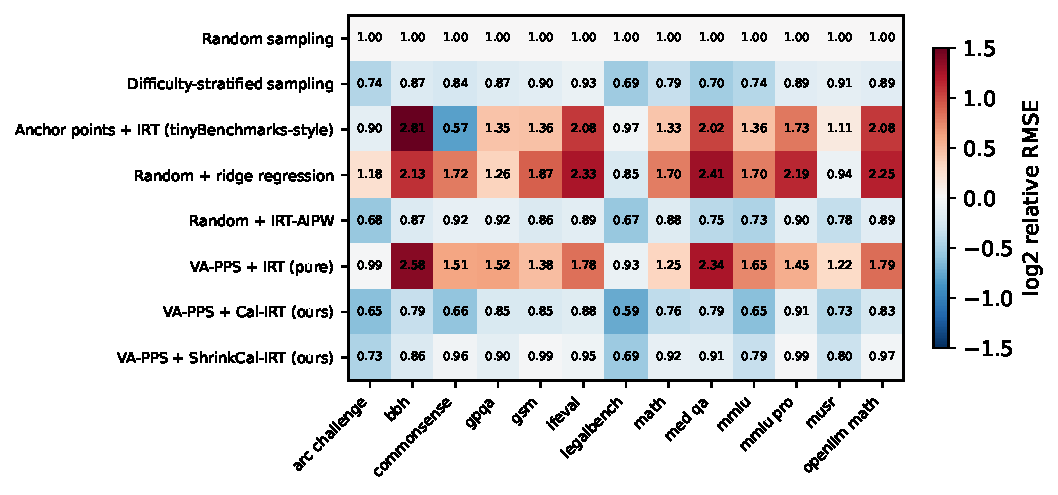
\includegraphics[width=0.95\linewidth]{figs/perbench_top100.pdf}
\caption{Per-benchmark relative RMSE at $n=100$, stronger-target split (cell values; colour = $\log_2$).}\label{fig:perbench}
\end{figure}
\begin{figure}[h]
\centering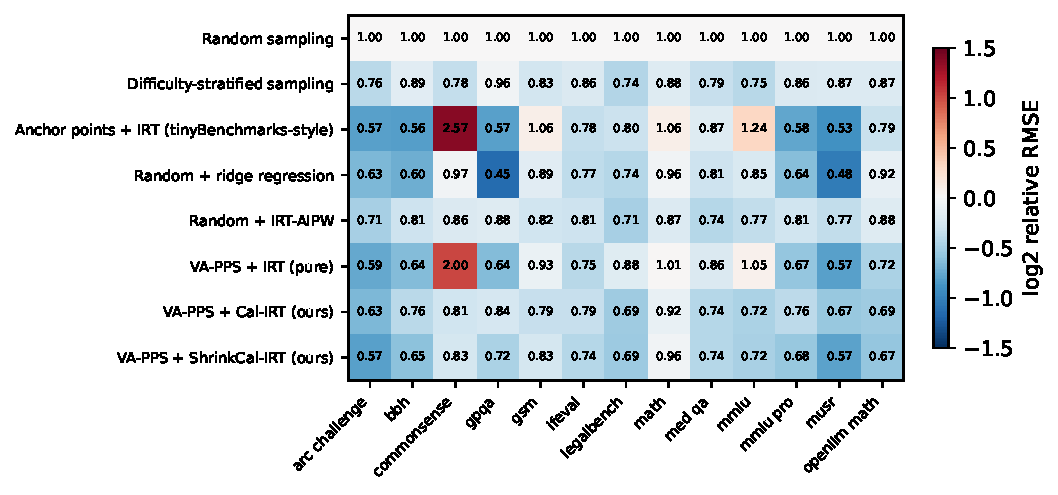
\includegraphics[width=0.95\linewidth]{figs/perbench_random100.pdf}
\caption{Per-benchmark relative RMSE at $n=100$, random split.}\label{fig:perbench2}
\end{figure}

\section{Shift severity}\label{app:shift}
Targets are the strongest 10\% / 25\% / 50\% or the weakest 25\% of models (by full-benchmark accuracy); the remaining models are sources. Ten seeds (0--9), $n\in\{25,100\}$, designs random, stratified, VA-PPS ($\lambda=1$) and anchors; the ``Stronger targets'' (25\%) column is the main-run result restricted to the same seeds.
\begin{table}[h]
\caption{Relative RMSE vs.\ random sampling under different shift severities (geometric mean over 13 benchmarks; 95\% hierarchical-bootstrap intervals).}\label{tab:shift}
\centering\tiny\setlength{\tabcolsep}{1.5pt}\resizebox{\linewidth}{!}{\begin{tabular}{lcccccccc}
\toprule
 & \multicolumn{2}{c}{Top-10\% targets} & \multicolumn{2}{c}{Stronger targets (extrapolation)} & \multicolumn{2}{c}{Top-50\% targets} & \multicolumn{2}{c}{Weakest-25\% targets} \\
 & $n$=25 & $n$=100 & $n$=25 & $n$=100 & $n$=25 & $n$=100 & $n$=25 & $n$=100 \\
\midrule
Random sampling & 1.00\,\scriptsize(1.00--1.00) & 1.00\,\scriptsize(1.00--1.00) & 1.00\,\scriptsize(1.00--1.00) & 1.00\,\scriptsize(1.00--1.00) & 1.00\,\scriptsize(1.00--1.00) & 1.00\,\scriptsize(1.00--1.00) & 1.00\,\scriptsize(1.00--1.00) & 1.00\,\scriptsize(1.00--1.00) \\
Difficulty-stratified sampling & 0.88\,\scriptsize(0.81--0.97) & 0.77\,\scriptsize(0.69--0.86) & 0.82\,\scriptsize(0.75--0.90) & 0.81\,\scriptsize(0.74--0.88) & 0.86\,\scriptsize(0.80--0.93) & 0.81\,\scriptsize(0.74--0.90) & 0.92\,\scriptsize(0.84--1.00) & 0.90\,\scriptsize(0.84--0.98) \\
Anchor points + IRT (tinyBenchmarks-style) & 0.96\,\scriptsize(0.80--1.19) & 1.00\,\scriptsize(0.74--1.30) & 1.02\,\scriptsize(0.85--1.24) & 1.37\,\scriptsize(1.09--1.74) & 1.34\,\scriptsize(1.11--1.67) & 1.97\,\scriptsize(1.61--2.50) & 1.36\,\scriptsize(0.98--1.87) & 2.16\,\scriptsize(1.47--3.15) \\
Random + ridge regression & 1.12\,\scriptsize(0.95--1.32) & 1.24\,\scriptsize(1.08--1.47) & 1.13\,\scriptsize(0.93--1.38) & 1.60\,\scriptsize(1.33--1.98) & 1.43\,\scriptsize(1.16--1.81) & 2.13\,\scriptsize(1.75--2.67) & 1.48\,\scriptsize(1.02--2.07) & 2.09\,\scriptsize(1.41--3.05) \\
Random + IRT-AIPW & 0.82\,\scriptsize(0.76--0.92) & 0.71\,\scriptsize(0.66--0.79) & 0.78\,\scriptsize(0.71--0.87) & 0.84\,\scriptsize(0.78--0.91) & 0.83\,\scriptsize(0.75--0.93) & 0.82\,\scriptsize(0.75--0.89) & 0.93\,\scriptsize(0.84--1.03) & 0.95\,\scriptsize(0.88--1.02) \\
VA-PPS + IRT (pure) & 1.00\,\scriptsize(0.84--1.22) & 1.16\,\scriptsize(1.04--1.36) & 1.03\,\scriptsize(0.87--1.25) & 1.48\,\scriptsize(1.28--1.77) & 1.33\,\scriptsize(1.11--1.62) & 2.07\,\scriptsize(1.77--2.49) & 1.38\,\scriptsize(1.00--1.84) & 2.12\,\scriptsize(1.50--2.99) \\
VA-PPS + Cal-IRT (ours) & 0.72\,\scriptsize(0.63--0.82) & 0.68\,\scriptsize(0.61--0.76) & 0.71\,\scriptsize(0.62--0.81) & 0.73\,\scriptsize(0.67--0.81) & 0.84\,\scriptsize(0.76--0.95) & 0.82\,\scriptsize(0.71--0.95) & 0.90\,\scriptsize(0.77--1.06) & 0.92\,\scriptsize(0.81--1.05) \\
VA-PPS + ShrinkCal-IRT (ours) & 0.83\,\scriptsize(0.72--0.98) & 0.80\,\scriptsize(0.73--0.91) & 0.81\,\scriptsize(0.71--0.94) & 0.85\,\scriptsize(0.79--0.93) & 0.95\,\scriptsize(0.84--1.09) & 0.93\,\scriptsize(0.82--1.07) & 1.01\,\scriptsize(0.84--1.20) & 1.07\,\scriptsize(0.93--1.24) \\
\bottomrule
\end{tabular}
}
\end{table}
\begin{table}[h]
\caption{Mean signed error (accuracy points, averaged over benchmarks) and bias$^2$/MSE at $n=100$ under different shifts.}\label{tab:shiftbias}
\centering\tiny\setlength{\tabcolsep}{1.5pt}\resizebox{\linewidth}{!}{\begin{tabular}{lcccccccc}
\toprule
 & \multicolumn{2}{c}{Top-10\% targets} & \multicolumn{2}{c}{Stronger targets (extrapolation)} & \multicolumn{2}{c}{Top-50\% targets} & \multicolumn{2}{c}{Weakest-25\% targets} \\
 & mean err (pts) & bias$^2$/MSE & mean err (pts) & bias$^2$/MSE & mean err (pts) & bias$^2$/MSE & mean err (pts) & bias$^2$/MSE \\
\midrule
Random sampling & -0.07 & 55\% & -0.55 & 41\% & -0.07 & 45\% & +0.04 & 26\% \\
Difficulty-stratified sampling & +0.10 & 26\% & -0.15 & 18\% & -0.12 & 16\% & -0.13 & 11\% \\
Anchor points + IRT (tinyBenchmarks-style) & -3.81 & 74\% & -5.01 & 72\% & -7.51 & 70\% & +9.01 & 70\% \\
Random + ridge regression & -4.43 & 81\% & -5.58 & 76\% & -7.99 & 73\% & +8.15 & 67\% \\
Random + IRT-AIPW & -0.20 & 17\% & -0.33 & 19\% & -0.31 & 21\% & +0.21 & 22\% \\
VA-PPS + IRT (pure) & -4.08 & 78\% & -5.17 & 76\% & -7.58 & 73\% & +8.23 & 69\% \\
VA-PPS + Cal-IRT (ours) & -0.63 & 25\% & -0.41 & 16\% & -0.74 & 24\% & +1.31 & 25\% \\
VA-PPS + ShrinkCal-IRT (ours) & -1.62 & 40\% & -1.44 & 29\% & -1.79 & 35\% & +2.28 & 40\% \\
\bottomrule
\end{tabular}
}
\end{table}


\section{Number of source models}\label{app:src}
Seven benchmarks (ARC-Challenge, GPQA, IFEval, MuSR, MATH Lvl 5, HELM MMLU, HELM GSM), seeds 0--9; $m$ source models drawn at random from the split's source set (``all'' = no subsampling; HELM splits have fewer than 100 sources, so $m=100$ equals ``all'' there). Relative RMSE vs.\ random sampling on the same targets (random sampling does not depend on $m$).
\begin{table}[h]
\caption{Relative RMSE vs.\ number of source models $m$, $n=25$.}\label{tab:src25}
\centering\tiny\setlength{\tabcolsep}{1.5pt}\resizebox{\linewidth}{!}{\begin{tabular}{lcccccccc}
\toprule
 & \multicolumn{4}{c}{Random split} & \multicolumn{4}{c}{Stronger targets} \\
 & $m$=20 & $m$=50 & $m$=100 & $m$=all & $m$=20 & $m$=50 & $m$=100 & $m$=all \\
\midrule
Difficulty-stratified sampling & 0.82\,\scriptsize(0.74--0.91) & 0.84\,\scriptsize(0.75--0.94) & 0.82\,\scriptsize(0.74--0.91) & 0.80\,\scriptsize(0.72--0.90) & 0.79\,\scriptsize(0.70--0.89) & 0.80\,\scriptsize(0.68--0.91) & 0.79\,\scriptsize(0.69--0.90) & 0.79\,\scriptsize(0.70--0.89) \\
VA-PPS + ridge regression & 0.71\,\scriptsize(0.52--0.95) & 0.56\,\scriptsize(0.42--0.74) & 0.52\,\scriptsize(0.38--0.70) & 0.51\,\scriptsize(0.37--0.69) & 1.22\,\scriptsize(0.88--1.70) & 1.05\,\scriptsize(0.75--1.47) & 0.97\,\scriptsize(0.70--1.30) & 0.96\,\scriptsize(0.70--1.30) \\
VA-PPS + IRT (pure) & 0.77\,\scriptsize(0.55--1.02) & 0.61\,\scriptsize(0.46--0.79) & 0.55\,\scriptsize(0.43--0.72) & 0.56\,\scriptsize(0.43--0.72) & 1.47\,\scriptsize(1.04--2.06) & 1.14\,\scriptsize(0.83--1.55) & 1.01\,\scriptsize(0.75--1.31) & 0.87\,\scriptsize(0.69--1.12) \\
VA-PPS + IRT-AIPW & 0.96\,\scriptsize(0.80--1.15) & 0.82\,\scriptsize(0.70--0.97) & 0.71\,\scriptsize(0.62--0.82) & 0.73\,\scriptsize(0.63--0.84) & 1.51\,\scriptsize(0.92--2.06) & 0.97\,\scriptsize(0.66--1.37) & 0.84\,\scriptsize(0.63--1.11) & 0.79\,\scriptsize(0.65--0.96) \\
VA-PPS + Cal-IRT & 0.71\,\scriptsize(0.58--0.86) & 0.65\,\scriptsize(0.54--0.77) & 0.63\,\scriptsize(0.53--0.74) & 0.64\,\scriptsize(0.54--0.75) & 0.86\,\scriptsize(0.67--1.07) & 0.76\,\scriptsize(0.61--0.95) & 0.74\,\scriptsize(0.60--0.91) & 0.68\,\scriptsize(0.56--0.81) \\
VA-PPS + ShrinkCal-IRT & 0.70\,\scriptsize(0.54--0.88) & 0.62\,\scriptsize(0.50--0.75) & 0.57\,\scriptsize(0.46--0.69) & 0.58\,\scriptsize(0.47--0.71) & 0.98\,\scriptsize(0.77--1.22) & 0.87\,\scriptsize(0.67--1.10) & 0.81\,\scriptsize(0.64--0.98) & 0.73\,\scriptsize(0.59--0.91) \\
\bottomrule
\end{tabular}
}
\end{table}
\begin{table}[h]
\caption{Relative RMSE vs.\ number of source models $m$, $n=100$.}\label{tab:src100}
\centering\tiny\setlength{\tabcolsep}{1.5pt}\resizebox{\linewidth}{!}{\begin{tabular}{lcccccccc}
\toprule
 & \multicolumn{4}{c}{Random split} & \multicolumn{4}{c}{Stronger targets} \\
 & $m$=20 & $m$=50 & $m$=100 & $m$=all & $m$=20 & $m$=50 & $m$=100 & $m$=all \\
\midrule
Difficulty-stratified sampling & 0.86\,\scriptsize(0.78--0.96) & 0.83\,\scriptsize(0.76--0.91) & 0.85\,\scriptsize(0.77--0.93) & 0.83\,\scriptsize(0.75--0.91) & 0.83\,\scriptsize(0.73--0.92) & 0.82\,\scriptsize(0.74--0.90) & 0.84\,\scriptsize(0.77--0.93) & 0.83\,\scriptsize(0.74--0.92) \\
VA-PPS + ridge regression & 0.92\,\scriptsize(0.75--1.10) & 0.75\,\scriptsize(0.62--0.89) & 0.75\,\scriptsize(0.61--0.91) & 0.66\,\scriptsize(0.53--0.82) & 1.96\,\scriptsize(1.43--2.81) & 1.71\,\scriptsize(1.30--2.30) & 1.60\,\scriptsize(1.25--2.12) & 1.42\,\scriptsize(1.10--1.83) \\
VA-PPS + IRT (pure) & 1.25\,\scriptsize(1.00--1.49) & 0.86\,\scriptsize(0.72--1.01) & 0.80\,\scriptsize(0.66--0.95) & 0.71\,\scriptsize(0.61--0.83) & 2.63\,\scriptsize(1.98--3.70) & 1.96\,\scriptsize(1.48--2.62) & 1.70\,\scriptsize(1.34--2.18) & 1.40\,\scriptsize(1.20--1.60) \\
VA-PPS + IRT-AIPW & 1.12\,\scriptsize(1.00--1.24) & 0.85\,\scriptsize(0.73--1.00) & 0.83\,\scriptsize(0.74--0.93) & 0.78\,\scriptsize(0.69--0.89) & 1.16\,\scriptsize(0.92--1.51) & 0.96\,\scriptsize(0.74--1.24) & 0.87\,\scriptsize(0.73--1.04) & 0.82\,\scriptsize(0.69--0.96) \\
VA-PPS + Cal-IRT & 0.84\,\scriptsize(0.71--0.95) & 0.75\,\scriptsize(0.65--0.84) & 0.76\,\scriptsize(0.67--0.85) & 0.73\,\scriptsize(0.65--0.82) & 0.94\,\scriptsize(0.75--1.22) & 0.85\,\scriptsize(0.70--1.04) & 0.81\,\scriptsize(0.65--1.00) & 0.73\,\scriptsize(0.63--0.83) \\
VA-PPS + ShrinkCal-IRT & 0.86\,\scriptsize(0.74--0.97) & 0.71\,\scriptsize(0.61--0.82) & 0.72\,\scriptsize(0.62--0.84) & 0.68\,\scriptsize(0.60--0.77) & 1.10\,\scriptsize(0.92--1.34) & 0.95\,\scriptsize(0.83--1.12) & 0.90\,\scriptsize(0.75--1.07) & 0.82\,\scriptsize(0.73--0.93) \\
\bottomrule
\end{tabular}
}
\end{table}

\section{Reproducibility and disclosures}\label{app:repro}
\textbf{Code and commands.} See \texttt{README.md} in the supplementary code. In short: \texttt{run\_exp.py --tag main --seeds 0-29 --budgets 10,25,50,100,200 --auto --jobs 4} (main grid, 990 jobs, about 3.5\,h on 4 CPU cores), \texttt{run\_exp.py --tag shift --protocols top10,top50,bottom --seeds 0-9 --budgets 25,100 --designs rand,strat,pps1.0,anchor} (shift-severity run), and the source-size runs (\texttt{run\_exp.py --tag src$K$ --benchmarks arc\_challenge,gpqa,ifeval,musr,openllm\_math,mmlu,gsm --protocols random,top --seeds 0-9 --budgets 25,100 --designs strat,pps1.0 --max\_sources $K$}, $K\in\{20,50,100\}$); then \texttt{analyze.py main}, \texttt{analyze.py shift} and \texttt{analyze\_src.py} regenerate all tables and figures. Re-running two main-grid jobs (IFEval and GSM, stronger-target split, seed 3) reproduced all stored results exactly (maximum absolute difference 0). Software: Python 3.11, numpy 2.4.6, scipy 1.17.1, scikit-learn 1.9.1, pandas 3.1.0, joblib 1.6.0, matplotlib 3.11.2. Randomness: split seed $s$ uses \texttt{default\_rng(10000+s)}; coreset/IRT-initialisation randomness uses \texttt{default\_rng(s)}; AUTO inner splits use \texttt{default\_rng(777000+s)}. Development runs used seeds $\ge1000$ (and 2000--2007) and are not part of the reported tables.\\
\textbf{Data.} Files \texttt{data/scores/*.jbl} from \url{https://github.com/socialfoundations/benchmark-prediction} at commit \texttt{55faff496947789f94e6b5908c77cbc3e84f81ad} (SHA-256 sums of all files are recorded in \texttt{data/SHA256SUMS.txt}). We only used the score matrices and model lists; we did not use the \texttt{benchpred} package, nor re-run any model. Upstream sources: Open LLM Leaderboard v2, HELM.\\
\textbf{Related-work disclosure.} Regarding the restriction on reading the paper that studies this exact problem: we did not search for, open or read any paper on that topic apart from the items of the provided starter list. The starter list includes the NeurIPS 2025 paper of \citet{zhang2025misses}; we did \emph{not} read it. Our knowledge of it is limited to its description in the starter list and the README of the data repository (which we read when downloading the data and which summarises its conclusions in three sentences, quoted in spirit in Section~\ref{sec:related}). Other literature was located through a scholarly-search tool (titles and abstract snippets only) to verify citation details. No other encounter with restricted content occurred.\\
\textbf{Use of an AI agent.} All code, experiments, analysis and text of this study were produced by an autonomous AI research agent (Claude Sonnet 5.5, Claude Agent SDK) running unattended.\\
\textbf{Failed or abandoned items.} The first launch of the main run used 38 worker processes under a 4-core CPU quota and was killed and restarted with 4 workers before producing any result file. The cross-fitted AIPW variant (\texttt{gregcf}) was worse than in-sample AIPW and is reported in Table~\ref{tab:abl} only. On the development run, weaker item regularisation (0.2 instead of 1) was slightly worse for Cal-IRT and larger ability-prior variances (25, 1000) were similar or worse, so neither was adopted; extra Platt penalties (5, 20) and an intercept-only recalibration were not better than the default either.


\newpage
\section*{NeurIPS Paper Checklist}




\begin{enumerate}

\item {\bf Claims}
    \item[] Question: Do the main claims made in the abstract and introduction accurately reflect the paper's contributions and scope?
    \item[] Answer: \answerYes{} % Replace by \answerYes{}, \answerNo{}, or \answerNA{}.
    \item[] Justification: The abstract and introduction state the scope (13 binary item-level benchmarks, three split types), the components proposed, and the negative findings (uncorrected predictors fail under extrapolation, pseudo-shift tuning does not help); Section~\ref{sec:results} supports each claim.
    \item[] Guidelines:
    \begin{itemize}
        \item The answer \answerNA{} means that the abstract and introduction do not include the claims made in the paper.
        \item The abstract and/or introduction should clearly state the claims made, including the contributions made in the paper and important assumptions and limitations. A \answerNo{} or \answerNA{} answer to this question will not be perceived well by the reviewers. 
        \item The claims made should match theoretical and experimental results, and reflect how much the results can be expected to generalize to other settings. 
        \item It is fine to include aspirational goals as motivation as long as it is clear that these goals are not attained by the paper. 
    \end{itemize}

\item {\bf Limitations}
    \item[] Question: Does the paper discuss the limitations of the work performed by the authors?
    \item[] Answer: \answerYes{} % Replace by \answerYes{}, \answerNo{}, or \answerNA{}.
    \item[] Justification: Section~\ref{sec:discussion} lists limitations (scope, shift operationalisation, re-implemented baselines, tuning, lack of guarantees).
    \item[] Guidelines:
    \begin{itemize}
        \item The answer \answerNA{} means that the paper has no limitation while the answer \answerNo{} means that the paper has limitations, but those are not discussed in the paper. 
        \item The authors are encouraged to create a separate ``Limitations'' section in their paper.
        \item The paper should point out any strong assumptions and how robust the results are to violations of these assumptions (e.g., independence assumptions, noiseless settings, model well-specification, asymptotic approximations only holding locally). The authors should reflect on how these assumptions might be violated in practice and what the implications would be.
        \item The authors should reflect on the scope of the claims made, e.g., if the approach was only tested on a few datasets or with a few runs. In general, empirical results often depend on implicit assumptions, which should be articulated.
        \item The authors should reflect on the factors that influence the performance of the approach. For example, a facial recognition algorithm may perform poorly when image resolution is low or images are taken in low lighting. Or a speech-to-text system might not be used reliably to provide closed captions for online lectures because it fails to handle technical jargon.
        \item The authors should discuss the computational efficiency of the proposed algorithms and how they scale with dataset size.
        \item If applicable, the authors should discuss possible limitations of their approach to address problems of privacy and fairness.
        \item While the authors might fear that complete honesty about limitations might be used by reviewers as grounds for rejection, a worse outcome might be that reviewers discover limitations that aren't acknowledged in the paper. The authors should use their best judgment and recognize that individual actions in favor of transparency play an important role in developing norms that preserve the integrity of the community. Reviewers will be specifically instructed to not penalize honesty concerning limitations.
    \end{itemize}

\item {\bf Theory assumptions and proofs}
    \item[] Question: For each theoretical result, does the paper provide the full set of assumptions and a complete (and correct) proof?
    \item[] Answer: \answerYes{} % Replace by \answerYes{}, \answerNo{}, or \answerNA{}.
    \item[] Justification: Proposition~\ref{prop:neyman} states its assumptions and has a short complete proof; the heuristics (Cal-IRT, ShrinkCal-IRT, VA-PPS proxy) are explicitly presented without guarantees.
    \item[] Guidelines:
    \begin{itemize}
        \item The answer \answerNA{} means that the paper does not include theoretical results. 
        \item All the theorems, formulas, and proofs in the paper should be numbered and cross-referenced.
        \item All assumptions should be clearly stated or referenced in the statement of any theorems.
        \item The proofs can either appear in the main paper or the supplemental material, but if they appear in the supplemental material, the authors are encouraged to provide a short proof sketch to provide intuition. 
        \item Inversely, any informal proof provided in the core of the paper should be complemented by formal proofs provided in appendix or supplemental material.
        \item Theorems and Lemmas that the proof relies upon should be properly referenced. 
    \end{itemize}

    \item {\bf Experimental result reproducibility}
    \item[] Question: Does the paper fully disclose all the information needed to reproduce the main experimental results of the paper to the extent that it affects the main claims and/or conclusions of the paper (regardless of whether the code and data are provided or not)?
    \item[] Answer: \answerYes{} % Replace by \answerYes{}, \answerNo{}, or \answerNA{}.
    \item[] Justification: Sections~\ref{sec:method}--\ref{sec:protocol} and Appendix~\ref{app:impl} specify designs, estimators, splits, budgets, seeds and hyper-parameters; the README gives exact commands.
    \item[] Guidelines:
    \begin{itemize}
        \item The answer \answerNA{} means that the paper does not include experiments.
        \item If the paper includes experiments, a \answerNo{} answer to this question will not be perceived well by the reviewers: Making the paper reproducible is important, regardless of whether the code and data are provided or not.
        \item If the contribution is a dataset and\slash or model, the authors should describe the steps taken to make their results reproducible or verifiable. 
        \item Depending on the contribution, reproducibility can be accomplished in various ways. For example, if the contribution is a novel architecture, describing the architecture fully might suffice, or if the contribution is a specific model and empirical evaluation, it may be necessary to either make it possible for others to replicate the model with the same dataset, or provide access to the model. In general. releasing code and data is often one good way to accomplish this, but reproducibility can also be provided via detailed instructions for how to replicate the results, access to a hosted model (e.g., in the case of a large language model), releasing of a model checkpoint, or other means that are appropriate to the research performed.
        \item While NeurIPS does not require releasing code, the conference does require all submissions to provide some reasonable avenue for reproducibility, which may depend on the nature of the contribution. For example
        \begin{enumerate}
            \item If the contribution is primarily a new algorithm, the paper should make it clear how to reproduce that algorithm.
            \item If the contribution is primarily a new model architecture, the paper should describe the architecture clearly and fully.
            \item If the contribution is a new model (e.g., a large language model), then there should either be a way to access this model for reproducing the results or a way to reproduce the model (e.g., with an open-source dataset or instructions for how to construct the dataset).
            \item We recognize that reproducibility may be tricky in some cases, in which case authors are welcome to describe the particular way they provide for reproducibility. In the case of closed-source models, it may be that access to the model is limited in some way (e.g., to registered users), but it should be possible for other researchers to have some path to reproducing or verifying the results.
        \end{enumerate}
    \end{itemize}


\item {\bf Open access to data and code}
    \item[] Question: Does the paper provide open access to the data and code, with sufficient instructions to faithfully reproduce the main experimental results, as described in supplemental material?
    \item[] Answer: \answerYes{} % Replace by \answerYes{}, \answerNo{}, or \answerNA{}.
    \item[] Justification: Data are public (fixed commit, MIT licence); all code, including the script generating each table/figure, is supplied (README, Appendix~\ref{app:repro}).
    \item[] Guidelines:
    \begin{itemize}
        \item The answer \answerNA{} means that paper does not include experiments requiring code.
        \item Please see the NeurIPS code and data submission guidelines (\url{https://neurips.cc/public/guides/CodeSubmissionPolicy}) for more details.
        \item While we encourage the release of code and data, we understand that this might not be possible, so \answerNo{} is an acceptable answer. Papers cannot be rejected simply for not including code, unless this is central to the contribution (e.g., for a new open-source benchmark).
        \item The instructions should contain the exact command and environment needed to run to reproduce the results. See the NeurIPS code and data submission guidelines (\url{https://neurips.cc/public/guides/CodeSubmissionPolicy}) for more details.
        \item The authors should provide instructions on data access and preparation, including how to access the raw data, preprocessed data, intermediate data, and generated data, etc.
        \item The authors should provide scripts to reproduce all experimental results for the new proposed method and baselines. If only a subset of experiments are reproducible, they should state which ones are omitted from the script and why.
        \item At submission time, to preserve anonymity, the authors should release anonymized versions (if applicable).
        \item Providing as much information as possible in supplemental material (appended to the paper) is recommended, but including URLs to data and code is permitted.
    \end{itemize}


\item {\bf Experimental setting/details}
    \item[] Question: Does the paper specify all the training and test details (e.g., data splits, hyperparameters, how they were chosen, type of optimizer) necessary to understand the results?
    \item[] Answer: \answerYes{} % Replace by \answerYes{}, \answerNo{}, or \answerNA{}.
    \item[] Justification: No training in the usual sense; splits, budgets, seeds, IRT/optimiser settings and how hyper-parameters were chosen (separate development run) are given in Section~\ref{sec:protocol} and Appendix~\ref{app:impl}.
    \item[] Guidelines:
    \begin{itemize}
        \item The answer \answerNA{} means that the paper does not include experiments.
        \item The experimental setting should be presented in the core of the paper to a level of detail that is necessary to appreciate the results and make sense of them.
        \item The full details can be provided either with the code, in appendix, or as supplemental material.
    \end{itemize}

\item {\bf Experiment statistical significance}
    \item[] Question: Does the paper report error bars suitably and correctly defined or other appropriate information about the statistical significance of the experiments?
    \item[] Answer: \answerYes{} % Replace by \answerYes{}, \answerNo{}, or \answerNA{}.
    \item[] Justification: 95\% hierarchical bootstrap intervals (resampling benchmarks, then seeds) for every aggregate and paired comparison; what the intervals do and do not cover is stated in Section~\ref{sec:protocol}.
    \item[] Guidelines:
    \begin{itemize}
        \item The answer \answerNA{} means that the paper does not include experiments.
        \item The authors should answer \answerYes{} if the results are accompanied by error bars, confidence intervals, or statistical significance tests, at least for the experiments that support the main claims of the paper.
        \item The factors of variability that the error bars are capturing should be clearly stated (for example, train/test split, initialization, random drawing of some parameter, or overall run with given experimental conditions).
        \item The method for calculating the error bars should be explained (closed form formula, call to a library function, bootstrap, etc.)
        \item The assumptions made should be given (e.g., Normally distributed errors).
        \item It should be clear whether the error bar is the standard deviation or the standard error of the mean.
        \item It is OK to report 1-sigma error bars, but one should state it. The authors should preferably report a 2-sigma error bar than state that they have a 96\% CI, if the hypothesis of Normality of errors is not verified.
        \item For asymmetric distributions, the authors should be careful not to show in tables or figures symmetric error bars that would yield results that are out of range (e.g., negative error rates).
        \item If error bars are reported in tables or plots, the authors should explain in the text how they were calculated and reference the corresponding figures or tables in the text.
    \end{itemize}

\item {\bf Experiments compute resources}
    \item[] Question: For each experiment, does the paper provide sufficient information on the computer resources (type of compute workers, memory, time of execution) needed to reproduce the experiments?
    \item[] Answer: \answerYes{} % Replace by \answerYes{}, \answerNo{}, or \answerNA{}.
    \item[] Justification: CPU only, 4 effective cores (cgroup limit), memory $<$ 1\,GB per process; wall-clock times are in Appendix~\ref{app:repro}.
    \item[] Guidelines:
    \begin{itemize}
        \item The answer \answerNA{} means that the paper does not include experiments.
        \item The paper should indicate the type of compute workers CPU or GPU, internal cluster, or cloud provider, including relevant memory and storage.
        \item The paper should provide the amount of compute required for each of the individual experimental runs as well as estimate the total compute. 
        \item The paper should disclose whether the full research project required more compute than the experiments reported in the paper (e.g., preliminary or failed experiments that didn't make it into the paper). 
    \end{itemize}
    
\item {\bf Code of ethics}
    \item[] Question: Does the research conducted in the paper conform, in every respect, with the NeurIPS Code of Ethics \url{https://neurips.cc/public/EthicsGuidelines}?
    \item[] Answer: \answerYes{} % Replace by \answerYes{}, \answerNo{}, or \answerNA{}.
    \item[] Justification: Only public, previously released model-evaluation records are used; no human subjects, no new data collection.
    \item[] Guidelines:
    \begin{itemize}
        \item The answer \answerNA{} means that the authors have not reviewed the NeurIPS Code of Ethics.
        \item If the authors answer \answerNo, they should explain the special circumstances that require a deviation from the Code of Ethics.
        \item The authors should make sure to preserve anonymity (e.g., if there is a special consideration due to laws or regulations in their jurisdiction).
    \end{itemize}


\item {\bf Broader impacts}
    \item[] Question: Does the paper discuss both potential positive societal impacts and negative societal impacts of the work performed?
    \item[] Answer: \answerYes{} % Replace by \answerYes{}, \answerNo{}, or \answerNA{}.
    \item[] Justification: Discussion paragraph on broader impact (cheaper evaluation vs.\ over-trusting predicted scores).
    \item[] Guidelines:
    \begin{itemize}
        \item The answer \answerNA{} means that there is no societal impact of the work performed.
        \item If the authors answer \answerNA{} or \answerNo, they should explain why their work has no societal impact or why the paper does not address societal impact.
        \item Examples of negative societal impacts include potential malicious or unintended uses (e.g., disinformation, generating fake profiles, surveillance), fairness considerations (e.g., deployment of technologies that could make decisions that unfairly impact specific groups), privacy considerations, and security considerations.
        \item The conference expects that many papers will be foundational research and not tied to particular applications, let alone deployments. However, if there is a direct path to any negative applications, the authors should point it out. For example, it is legitimate to point out that an improvement in the quality of generative models could be used to generate Deepfakes for disinformation. On the other hand, it is not needed to point out that a generic algorithm for optimizing neural networks could enable people to train models that generate Deepfakes faster.
        \item The authors should consider possible harms that could arise when the technology is being used as intended and functioning correctly, harms that could arise when the technology is being used as intended but gives incorrect results, and harms following from (intentional or unintentional) misuse of the technology.
        \item If there are negative societal impacts, the authors could also discuss possible mitigation strategies (e.g., gated release of models, providing defenses in addition to attacks, mechanisms for monitoring misuse, mechanisms to monitor how a system learns from feedback over time, improving the efficiency and accessibility of ML).
    \end{itemize}
    
\item {\bf Safeguards}
    \item[] Question: Does the paper describe safeguards that have been put in place for responsible release of data or models that have a high risk for misuse (e.g., pre-trained language models, image generators, or scraped datasets)?
    \item[] Answer: \answerNA{} % Replace by \answerYes{}, \answerNo{}, or \answerNA{}.
    \item[] Justification: No models or datasets with high misuse risk are released.
    \item[] Guidelines:
    \begin{itemize}
        \item The answer \answerNA{} means that the paper poses no such risks.
        \item Released models that have a high risk for misuse or dual-use should be released with necessary safeguards to allow for controlled use of the model, for example by requiring that users adhere to usage guidelines or restrictions to access the model or implementing safety filters. 
        \item Datasets that have been scraped from the Internet could pose safety risks. The authors should describe how they avoided releasing unsafe images.
        \item We recognize that providing effective safeguards is challenging, and many papers do not require this, but we encourage authors to take this into account and make a best faith effort.
    \end{itemize}

\item {\bf Licenses for existing assets}
    \item[] Question: Are the creators or original owners of assets (e.g., code, data, models), used in the paper, properly credited and are the license and terms of use explicitly mentioned and properly respected?
    \item[] Answer: \answerYes{} % Replace by \answerYes{}, \answerNo{}, or \answerNA{}.
    \item[] Justification: The data come from the benchmark-prediction repository of \citet{zhang2025misses} (MIT licence, fixed commit) built from the Open LLM Leaderboard and HELM, both credited; upstream terms are noted in Appendix~\ref{app:repro}.
    \item[] Guidelines:
    \begin{itemize}
        \item The answer \answerNA{} means that the paper does not use existing assets.
        \item The authors should cite the original paper that produced the code package or dataset.
        \item The authors should state which version of the asset is used and, if possible, include a URL.
        \item The name of the license (e.g., CC-BY 4.0) should be included for each asset.
        \item For scraped data from a particular source (e.g., website), the copyright and terms of service of that source should be provided.
        \item If assets are released, the license, copyright information, and terms of use in the package should be provided. For popular datasets, \url{paperswithcode.com/datasets} has curated licenses for some datasets. Their licensing guide can help determine the license of a dataset.
        \item For existing datasets that are re-packaged, both the original license and the license of the derived asset (if it has changed) should be provided.
        \item If this information is not available online, the authors are encouraged to reach out to the asset's creators.
    \end{itemize}

\item {\bf New assets}
    \item[] Question: Are new assets introduced in the paper well documented and is the documentation provided alongside the assets?
    \item[] Answer: \answerYes{} % Replace by \answerYes{}, \answerNo{}, or \answerNA{}.
    \item[] Justification: The released asset is the code; it is documented in the README. No new datasets.
    \item[] Guidelines:
    \begin{itemize}
        \item The answer \answerNA{} means that the paper does not release new assets.
        \item Researchers should communicate the details of the dataset\slash code\slash model as part of their submissions via structured templates. This includes details about training, license, limitations, etc. 
        \item The paper should discuss whether and how consent was obtained from people whose asset is used.
        \item At submission time, remember to anonymize your assets (if applicable). You can either create an anonymized URL or include an anonymized zip file.
    \end{itemize}

\item {\bf Crowdsourcing and research with human subjects}
    \item[] Question: For crowdsourcing experiments and research with human subjects, does the paper include the full text of instructions given to participants and screenshots, if applicable, as well as details about compensation (if any)? 
    \item[] Answer: \answerNA{} % Replace by \answerYes{}, \answerNo{}, or \answerNA{}.
    \item[] Justification: No crowdsourcing or human subjects.
    \item[] Guidelines:
    \begin{itemize}
        \item The answer \answerNA{} means that the paper does not involve crowdsourcing nor research with human subjects.
        \item Including this information in the supplemental material is fine, but if the main contribution of the paper involves human subjects, then as much detail as possible should be included in the main paper. 
        \item According to the NeurIPS Code of Ethics, workers involved in data collection, curation, or other labor should be paid at least the minimum wage in the country of the data collector. 
    \end{itemize}

\item {\bf Institutional review board (IRB) approvals or equivalent for research with human subjects}
    \item[] Question: Does the paper describe potential risks incurred by study participants, whether such risks were disclosed to the subjects, and whether Institutional Review Board (IRB) approvals (or an equivalent approval/review based on the requirements of your country or institution) were obtained?
    \item[] Answer: \answerNA{} % Replace by \answerYes{}, \answerNo{}, or \answerNA{}.
    \item[] Justification: No human subjects.
    \item[] Guidelines:
    \begin{itemize}
        \item The answer \answerNA{} means that the paper does not involve crowdsourcing nor research with human subjects.
        \item Depending on the country in which research is conducted, IRB approval (or equivalent) may be required for any human subjects research. If you obtained IRB approval, you should clearly state this in the paper. 
        \item We recognize that the procedures for this may vary significantly between institutions and locations, and we expect authors to adhere to the NeurIPS Code of Ethics and the guidelines for their institution. 
        \item For initial submissions, do not include any information that would break anonymity (if applicable), such as the institution conducting the review.
    \end{itemize}

\item {\bf Declaration of LLM usage}
    \item[] Question: Does the paper describe the usage of LLMs if it is an important, original, or non-standard component of the core methods in this research? Note that if the LLM is used only for writing, editing, or formatting purposes and does \emph{not} impact the core methodology, scientific rigor, or originality of the research, declaration is not required.
    %this research? 
    \item[] Answer: \answerYes{} % Replace by \answerYes{}, \answerNo{}, or \answerNA{}.
    \item[] Justification: No LLM is part of the method; the whole study (code, experiments, analysis, writing) was carried out by an autonomous LLM agent (Claude Sonnet 5.5 via the Claude Agent SDK), disclosed in Appendix~\ref{app:repro}.
    \item[] Guidelines:
    \begin{itemize}
        \item The answer \answerNA{} means that the core method development in this research does not involve LLMs as any important, original, or non-standard components.
        \item Please refer to our LLM policy in the NeurIPS handbook for what should or should not be described.
    \end{itemize}

\end{enumerate}
\end{document}
